% \iffalse meta-comment
% Copyright (C) 2006-2009 by Martin Scharrer <martin@scharrer-online.de>
% http://latex.scharrer-online.de/svn-multi/
% -----------------------------------------------------------------
%
% This work may be distributed and/or modified under the
% conditions of the LaTeX Project Public License, either version 1.3
% of this license or (at your option) any later version.
% The latest version of this license is in
%   http://www.latex-project.org/lppl.txt
% and version 1.3 or later is part of all distributions of LaTeX
% version 2005/12/01 or later.
%
% This work has the LPPL maintenance status `maintained'.
%
% The Current Maintainer of this work is Martin Scharrer.
%
% This work consists of the files svn-multi.dtx and svn-multi.ins
% and the derived files svn-multi.sty and svnkw.sty.
%
% <*driver>
\makeatletter
% </driver>
% \fi
% \iffalse
%<*package|driver>
% $Id$
%
\def\svnmulti@version{v2.3-dev}
\RequirePackage{svn-prov}
%</package|driver>
%<*driver>
\ProvidesFileSVN{$Id$}
 [\svnmulti@version\space SVN Keywords for multi-file LaTeX documents]
\GetFileInfoSVN*
\let\svnmulti@date\filedate
\let\svnmulti@rev\filerev

\documentclass{ltxdoc}
\usepackage[english]{babel}
\dateenglish

\def\svnmulti@today#1/#2/#3\relax{%
  \begingroup
    \year#1\relax
    \month#2\relax
    \day#3\relax
    \xdef\svnmulti@today{\today}
  \endgroup
}
\expandafter\svnmulti@today\svnmulti@date\relax

\usepackage{svn-multi}[\svnmulti@date]
\usepackage{booktabs}
\usepackage{ifpdf}
\ifpdf
  % use hypdoc if you have it, hyperref else
  \IfFileExists{hypdoc.sty}
    {\usepackage{hypdoc}}
    {\usepackage{hyperref}}
\else
  \let\url\texttt
\fi
\usepackage{xspace}
\newcommand{\ie}{i.e.\@\xspace}
\newcommand{\eg}{e.g.\@\xspace}

\iffalse
\let\css=\cs
\let\op=\cs
\let\DescribeOption\DescribeMacro
\let\DescribeScript\DescribeOption
\else % crossreference of macros in documentation
\makeatletter

\usepackage{xspace}
\@namedef{seen@package@latex}{1} %^^A avoid footnotes for 'latex'
\newcommand*{\pkg}[1]{%
  \href{http://tug.ctan.org/pkg/#1}{\texttt{#1}}%
  % URL footnote (for print-out) on first appearance:
  \@ifundefined{seen@package@#1}{%
    \footnote{CTAN: \url{http://tug.ctan.org/pkg/#1}}%
    \@namedef{seen@package@#1}{1}%
  }{}%
  \xspace
}
\newcommand*{\svnmulti}{%
  \texttt{svn-multi}\xspace%
}

% link \cs to macro definitions
\let\origmacro\macro
\let\origendmacro\endmacro
\let\origStopEventually\StopEventually
\let\origPrintDescribeMacro\PrintDescribeMacro
\usepackage{xcolor}
\definecolor{darkred}{rgb}{0.333,0.0,0.0}
\hypersetup{colorlinks=true,linkcolor=darkred,urlcolor=darkred}
\definecolor{macrodesccolor}{rgb}{0.0,0.0,0.8}
\definecolor{macroimplcolor}{rgb}{0.0,0.0,0.4}
\definecolor{metacolor}{rgb}{0.0,0.4,0.4}
\definecolor{scriptcolor}{rgb}{0.2,0.6,0.2}
\definecolor{optioncolor}{rgb}{0.3,0.2,0}

\let\macroline\\
\newlength{\macrosep}
\setlength{\macrosep}{-3em}
\renewcommand{\meta@font@select}{\color{metacolor}\itshape}
\newcommand{\macroformat}[1]{\textbf{\ttfamily #1}}
\newcommand{\optionformat}[1]{\textbf{\sffamily #1}}
\newcommand{\scriptformat}[1]{\textbf{\ttfamily #1}}
\newcommand{\macroargformat}[1]{\texttt{#1}}
\newcommand{\scriptargformat}[1]{\textbf{#1}}
\newcommand{\macrohlinkprefix}{desc}
\newcommand{\macrolink}{}

\usepackage[utf8]{inputenc}
\usepackage[T1]{fontenc}
\IfFileExists{lmodern.sty}{\usepackage{lmodern}}{}%

\def\DescribeMacro{\@ifnextchar*{\DescribeMacroS}{\DescribeMacroN}}
\def\DescribeMacroN{%
  \bigskip\pagebreak[3]\par\noindent\DescribeMacroS*%
}
\def\DescribeMacroS*#1#2{%
  \begingroup
  \g@namedef{href@desc@#1}{}%
  \immediate\write\@mainaux{%
    \noexpand\g@namedef{href@desc@#1}{}%
  }%
  \@ifundefined{href@impl@#1}%
    {\let\macrolink\relax}%
    {\def\macrolink{\hyperlink{impl@#1}}}%
  \hypersetup{linkcolor=macrodesccolor}%
  \hspace*{\macrosep}%
  \raisebox{\baselineskip}[\baselineskip]{\hypertarget{desc@#1}{}}%
  \macrolink{\macroformat{\textcolor{macrodesccolor}{\textbackslash #1}}}%
  \noindent\mbox{}\macroargformat{#2}\nopagebreak
  \macroline*[0.2\baselineskip]%
  \endgroup
  \nopagebreak
  \ignorespaces
}
\def\DescribeScript{\@ifnextchar*{\DescribeScriptS}{\DescribeScriptN}}
\def\DescribeScriptN{%
  \bigskip\par\pagebreak[2]\noindent\DescribeScriptS*%
}
\def\DescribeScriptS*#1#2{%
  \hspace*{\macrosep}%
  \raisebox{\baselineskip}[\baselineskip]{\hypertarget{script@#1}{}}%
  \scriptformat{\textcolor{scriptcolor}{#1}}%
  \noindent\mbox{}\scriptargformat{\ {#2}}\macroline*[0.2\baselineskip]%
  \nopagebreak
}
\def\DescribeOption{\@ifnextchar*{\DescribeOptionS}{\DescribeOptionN}}
\def\DescribeOptionN{%
  \bigskip\par\noindent\DescribeOptionS*%
}
\def\DescribeOptionS*#1{%
  \hspace*{\macrosep}%
  \raisebox{\baselineskip}[\baselineskip]{\hypertarget{option@#1}{}}%
  \optionformat{\textcolor{optioncolor}{#1}}%
  \noindent\mbox{}\macroline*[0.2\baselineskip]%
  \nopagebreak
}
\newcounter{macrolevel}
\renewenvironment{macro}[1]{%
  \addtocounter{macrolevel}{1}%
  \expandafter\macroX\expandafter{\expandafter\@gobble\string#1}%
}{%
  \addtocounter{macrolevel}{-1}%
}
\providecommand*{\g@namedef}[1]{%
  \expandafter\gdef\csname #1\endcsname
}
\newcommand*{\macroX}[1]{%
  \ifnum\c@macrolevel<2
    \smallskip
  \fi
  \par\noindent
  \g@namedef{href@impl@#1}{}%
  \immediate\write\@mainaux{%
    \noexpand\g@namedef{href@impl@#1}{}%
  }%
  \@ifundefined{href@desc@#1}%
    {\let\macrolink\relax}%
    {\def\macrolink{\hyperlink{desc@#1}}}%
  \hspace*{\macrosep}%
  \raisebox{\baselineskip}[\baselineskip]{\hypertarget{impl@#1}{}}%
  \macrolink{\macroformat{%
    \textcolor{macroimplcolor}{\textbackslash #1}}}%
  \\*[\smallskipamount]%
  \@ifnextchar\begin{\vspace*{-\baselineskip}}{\imacroarg}%
}

\newcounter{macroargs}
\newcounter{nmacroarg}

\newcommand*{\imacroarg}[1][0]{%
  \setcounter{macroargs}{#1}%
  \setcounter{nmacroarg}{1}%
  \ifnum\c@macroargs>0
    \expandafter\imacroargX
  \fi
}
\newcommand*{\aftermacroargs}{%
  \@ifnextchar\begin
    {\\*[-2ex]\ignorespaces}%
    {\\*[\smallskipamount]\ignorespaces}%
}
\newcommand*{\imacroargX}[1]{%
  \hspace*{-1em}\texttt{\#\thenmacroarg:} #1\relax
  \ifnum\c@macroargs>1
    \newline
  \fi
  \addtocounter{nmacroarg}{1}%
  \addtocounter{macroargs}{-1}%
  \ifnum\c@macroargs>0
    \expandafter\imacroargX
  \else
    \expandafter\aftermacroargs
  \fi
}


\def\karg#1{\{\$\textcolor{metacolor}{#1}\$\}}
\def\kmarg#1{\{\$\meta{#1}\$\}}

\DeclareRobustCommand{\csi}[1]{%
  \begingroup
  \hypersetup{linkcolor=macroimplcolor}%
  \renewcommand{\macrohlinkprefix}{impl}%
  \@ifundefined{href@impl@#1}%
    {\let\macrolink\relax}%
    {\def\macrolink{\hyperlink{impl@#1}}}%
  \csX{#1}%
  \endgroup
}
\DeclareRobustCommand{\csd}[1]{%
  \begingroup
  \hypersetup{linkcolor=macrodesccolor}%
  \renewcommand{\macrohlinkprefix}{macro}%
  \@ifundefined{href@desc@#1}%
    {\let\macrolink\relax}%
    {\def\macrolink{\hyperlink{desc@#1}}}%
  \csX{#1}%
  \endgroup
}
\DeclareRobustCommand{\csX}[1]{%
  \begingroup
  \macrolink{\texttt{\textbackslash#1}}%
  \endgroup
}
\let\cs\csd
\DeclareRobustCommand{\css}[1]{\texttt{\textbackslash#1}}
\DeclareRobustCommand{\op}[1]{%
  \begingroup
  \hypersetup{linkcolor=optioncolor}%
  \hyperlink{option@#1}{\textbf{\sffamily #1}}%
  \endgroup
}
\DeclareRobustCommand{\scr}[1]{%
  \begingroup
  \hypersetup{linkcolor=scriptcolor}%
  \hyperlink{script@#1}{\scriptformat{#1}}%
  \endgroup
}

\def\StopEventually#1{\origStopEventually{#1}%
\let\cs\csi
}

\fi

\usepackage{graphicx}

\EnableCrossrefs
%\DisableCrossrefs
\CodelineIndex
%\PageIndex
\RecordChanges
%\OnlyDescription
\widowpenalty=500
\clubpenalty=500
\listfiles
\begin{document}
  \DocInput{svn-multi.dtx}%
  \PrintChanges
  %\clearpage
  \PrintIndex
\end{document}
%</driver>
%<*package>
% \fi
%
% \CheckSum{2847}
%
% {\makeatother
% \CharacterTable
%  {Upper-case    \A\B\C\D\E\F\G\H\I\J\K\L\M\N\O\P\Q\R\S\T\U\V\W\X\Y\Z
%   Lower-case    \a\b\c\d\e\f\g\h\i\j\k\l\m\n\o\p\q\r\s\t\u\v\w\x\y\z
%   Digits        \0\1\2\3\4\5\6\7\8\9
%   Exclamation   \!     Double quote  \"     Hash (number) \#
%   Dollar        \$     Percent       \%     Ampersand     \&
%   Acute accent  \'     Left paren    \(     Right paren   \)
%   Asterisk      \*     Plus          \+     Comma         \,
%   Minus         \-     Point         \.     Solidus       \/
%   Colon         \:     Semicolon     \;     Less than     \<
%   Equals        \=     Greater than  \>     Question mark \?
%   Commercial at \@     Left bracket  \[     Backslash     \\
%   Right bracket \]     Circumflex    \^     Underscore    \_
%   Grave accent  \`     Left brace    \{     Vertical bar  \|
%   Right brace   \}     Tilde         \~}
% }
% \changes{v1.0}{2006/05/27}{Initial version}
% \changes{v1.1}{2006/06/08}{Added macros to extract and typeset date/time
% information. Added macros to set and typeset main URL or filename.}
% \changes{v1.2}{2007/06/22}{Renamed package from \texttt{svnkw} to
% \texttt{svn-multi} to match CTAN directory. Wrapper file
% \texttt{svnkw.sty} is provided for backward compatibility.}
% \changes{v1.3}{2007/07/01}{Added verbatim support. Keywords can now contain
% special character like \texttt{\_ \^{} \$ \% \& \textbackslash}. Rewrote
% keyword check macros to work with verbatim code. \texttt{\textbackslash
% nofiles} is now obeyed.}
% \changes{v1.3a}{2007/07/10}{Fixed issue with unwanted spaces generated by
% \cs{svnid}, \cs{svnidlong} and \cs{svnkwsave}, \eg when used in a file which
% is included with \css{input}}
% \changes{v1.3b}{2008/12/03}{Changed the way catcodes are modified to be
% compatible with the french option of the babel package or other packages which
% modify the list of special characters.}
% \changes{v1.4}{2009/02/27}{Added support for timezones with non-zero minute
% part, \eg +0530.}
% \changes{v1.5}{2009/02/28}{Added \css{today}-style macros \cs{svntoday} and
% \cs{svnfiletoday}.}
% \changes{v2.0}{2009/03/23}{New features: keyword groups, external file
% support, auto-include of images, files as subgroups and table of revisions.}
% \changes{v2.1}{2009/03/27}{Added automatic extraction of keywords from 
% Subversion 'entries' file: 'autokw' option}
% \changes{v2.2}{2009/10/19}{Added \css{ifsvnmodified} and 
% \css{ifsvnfilemodified} macros. Some bug fixes.}
% \changes{v2.3-dev}{2010/03/30}{Changed \css{svnidlong} to ignore all comments between verbatim arguments.}
%
% ^^A \GetFileInfo{svn-multi.dtx}
%
% \DoNotIndex{\newcommand,\newenvironment,\AtBeginDocument,\AtEndDocument}
% \DoNotIndex{\def,\let,\edef,\xdef,\item,\space,\write,\jobname,\relax,\!}
% \DoNotIndex{\closeout,\csname,\DeclareRobustCommand,\else,\empty,\newwrite}
% \DoNotIndex{\endcsname,\expandafter,\fi,\Hurl,\hyper@normalise,\@ifnextchar}
% \DoNotIndex{\ifnum,\@ifundefined,\ifx,\immediate,\InputIfFileExists,\ }
% \DoNotIndex{\newcount,\noexpand,\openout,\PackageWarning,\@percentchar}
% \DoNotIndex{\@sanitize,\@makeother,\@iwsvn,\%,\_,\&,\^,\$,\#,\ ,\\,\if@filesw}
% \DoNotIndex{\gdef,\begingroup,\endgroup,\catcode}
% \DoNotIndex{\^,\ ,\_,\(,\),\$,\&,\#,\@ampersamchar,\AtEndOfPackage}
% \DoNotIndex{\@backslashchar,\begin,\bgroup,\chapter,\day}
% \DoNotIndex{\DeclareOption,\do,\dospecials,\@dottedtocline,\egroup}
% \DoNotIndex{\end,\ExecuteOptions,\svnmulti@date,\svnmulti@version,\@for}
% \DoNotIndex{\futurelet,\g@addto@macro,\global,\@gobbletwo,\hline}
% \DoNotIndex{\hspace,\if@restonecol,\if@twocolumn,\ignorespaces}
% \DoNotIndex{\makeatletter,\MakeUppercase,\@mkboth,\month,\@namedef}
% \DoNotIndex{\NeedsTeXFormat,\newif,\onecolumn,\orig@fink@prepare}
% \DoNotIndex{\orig@fink@restore,\PackageError,\ProcessOptions}
% \DoNotIndex{\ProvidesPackage,\renewcommand,\RequirePackage}
% \DoNotIndex{\@restonecolfalse,\@restonecoltrue,\section,\strut}
% \DoNotIndex{\tableofcontents,\tableofrevisions,\texttt,\today}
% \DoNotIndex{\twocolumn,\@undefined,\url,\year}
% \DoNotIndex{\textwidth,\the,\string,\raggedright,\providecommand,\small,\toks@}
% \DoNotIndex{\medskipamount,\long,\leftskip,\clearpage,\advance,\addtolength}
% \DoNotIndex{\DeclareBoolOption,\DeclareStringOption,\DeclareVoidOption}
% \DoNotIndex{\ProcessKeyvalOptions,\SetupKeyvalOptions}
% \DoNotIndex{\@firstoftwo,\@secondoftwo,\@gobble}
%
% \title{The \textsf{svn-multi} Package \\\large formerly known as 
% \textsf{svnkw}}
% \author{Martin Scharrer \\ \url{martin@scharrer-online.de} \\
% \url{http://latex.scharrer-online.de/svn-multi/}\\
% CTAN: \url{http://tug.ctan.org/pkg/svn-multi}}
% \date{Version \expandafter\@gobble\svnmulti@version\\[0.5ex]\svnmulti@today}
%
% \ifpdf
% \hypersetup{%
%   pdfauthor   = {Martin Scharrer <martin@scharrer-online.de>},
%   pdftitle    = {The svn-multi package, \svnmulti@version, r\svnmulti@rev\ 
%                  from \svnmulti@date},
%   pdfsubject  = {Documentation of LaTeX package svn-multi which allows the 
%                  typesetting of Subversion keywords in multi-file LaTeX 
%                  documents},
%   pdfkeywords = {svn-multi, svnkw, LaTeX, Subversion, keywords, Version 
%                  Control, Id, Table Of Revisions}
% }%
% \fi
% \maketitle
%
% \vfill
%
% \section{Introduction}
% This package allows to typeset version control (VC) information provided by 
% Subversion\footnote{Subversion homepage: \url{http://subversion.tigris.org/}} 
% keywords (\eg |$||Id: ... $|) in \LaTeX\ documents which can contain of 
% multiple |.tex| files included using |\include| or |\input|.
% Subversion is a modern version control system designed to replace its 
% predecessor CVS and uses integers as revision numbers.
%
% This package reads the keywords of all files and provides the VC information 
% of of the most recent changed file of the document to the user through a set 
% of macros. This information is written to an auxiliary |.svn| file during the 
% first \LaTeX\ run and read back at the next which introduces the same delay 
% known from the table of contents. The standard \LaTeX{} switch |\nofiles| can 
% be used to suppress the file generation.
%
% In addition to this basic functionality several more features are provided:
% \begin{itemize}
%   \item Macros to typeset the VC information of the current source file.
%   \item Access of all parts of the VC date.
%   \item Formatting of author names or revision numbers.
%   \item Definition of groups and subgroups.
%   \item Including of the VC information of external files.
%   \item Table of Revisions.
% \end{itemize}
% \newpage
%
% \subsection{Scope of Keywords}
% This package provides the Subversion keyword data in several different scopes:
% document-global, file-local and, new with v2.0, by group.
%
% \subsubsection*{Document Global}
% The document global macros, like \cs{svnrev}, return the latest version 
% control information (keyword data) for the whole multi-file document, \ie the 
% information of the latest changed file of the document. To collect, sort and 
% provide this information is the main functionality of this package.
%
% \subsubsection*{Local to Current File}
% There are also file-local macros, \eg \cs{svnfilerev}, which return the 
% version control information of the current file, \ie the file they are used 
% in. It is assumed here that every file using this macros calls first either a 
% \cs{svnid} or \cs{svnidlong} macro or both.  See section~\ref{sec:usage:id} 
% for more details about the id macros.  Please note that the file-local macros 
% technically actually return the \emph{last registered} information from the 
% last \cs{svnid} or \cs{svnidlong}. As long the \op{filehooks} option (new in 
% v2.0) is not enabled (explicit or implicit) this keyword macros will leak from 
% one file over to the next.  This will cause wrong results if they are used in 
% a file before or without any id macros. With this option the macros will be 
% reset at the beginning of every source file of the document.
%
% \subsubsection*{Groups}
% Version 2.0 introduces the concept of groups. Several files of a multi-file 
% \LaTeX\ document can be grouped together and the latest version control 
% information of all files of a group is provided by macros. This works in the 
% same way as the global macros mentioned above but only with the files in the 
% group. It can also be seen from the other side: the macros are local like the 
% file-local macros mentioned above but for all files of the group, not only the 
% current one.
%
% These groups could also be called \textit{file groups}, \textit{keyword 
% groups} or, like in programming languages, \textit{namespaces}. In this manual 
% they will be reference as simple \textit{groups} most the time. In places 
% where they could be confused with \TeX\ groups (|{ }|, |\begingroup| 
% |\endgroup|), \eg ``in the current group'' or ``group local'', they will be 
% called \textit{keyword groups}.
%
% There is no limitation (besides internal \LaTeX\ resource limits) for the 
% number of different groups. The files of one group do not have to be included 
% in a row but can be included everywhere in the document. The version control 
% information of the current group can be typeset with macros like \cs{svncgrev} 
% (|cg| for \emph{current group}).  Also, a general but less robust macro 
% \cs{svng}\marg{group name}\marg{key} is provided to access others groups by 
% name everywhere in the document. To avoid some macro robustness problems the 
% current group can be changed locally for the output macros using 
% \cs{svnsetcg}\marg{group name}.
%
% See section~\ref{sec:group} for further details and usage instructions on 
% group macros.
%
% \section{Usage}
% The version control information are provided by Subversion keywords which
% first need to be read in by dedicated macros and can then be typeset using
% different macros.
%
% \subsection{Package Options}
% Since v2.0 this package provides options to enable only a needed features, \eg 
% to avoid problems with other packages or save \TeX\ memory. For backwards 
% compatibility to pre-2.0 package versions all old features are enabled by 
% default and all new features are disabled to save a little of \TeX\ memory.
%
% All options except the first two are boolean key=value options (so far) and
% await either `|true|' or `|false|' as value. A missing value means `|true|'.
% So \eg |[groups=true,verbatim=false,external]|, enables the \op{external} and
% \op{groups} options but disables the \op{verbatim} option.
%
% The available options are:\par
%
% \DescribeOption{old}
% Only pre-v2.0 features are active. This enables \op{verbatim} and disables all 
% other options below. This is the default for reasons mentioned above.
%
% \DescribeOption{all}
% Activates all features of the package except of the experimental ones.
%
% \DescribeOption{verbatim}
% Controls the verbatim mode of the keyword parser macros. Normally verbatim 
% mode is very much wanted to support strange characters in URLs and file names, 
% but this options gives the user a possibility to disable verbatim, \eg for 
% trouble shooting.  Please note that verbatim mode is needed in order to make 
% \svnmulti work with some packages, like \pkg{babel} with the |french| option.
%
% \DescribeOption{external}
% Controls the support for keywords from external files described in 
% section~\ref{sec:external}. This needs either the external script 
% \scr{svn-multi.pl} or the \op{autokw} option.
%
% If the \op{groups} option is enabled the macro 
% \csi{svnexternalgroup}\marg{group name} can be used to declare a own group 
% which is used for all the external files.  Otherwise they are placed in the 
% currently active group.  This macro can be used several times during the 
% document where an empty argument means \emph{no group} and a `|*|' means 
% \emph{current group}.
%
% \DescribeOption{groups}
% Controls the keyword groups feature described in section~\ref{sec:group}.
%
% \DescribeOption{subgroups}
% Controls the automatic declaration of all input files as subgroups so that 
% there keyword information can be typeset inside other files. The group name is 
% the file path without the file extension (`|subdir/filebase|').
% It is possible to disable and re-enable this using \cs{svnsubgroupsfalse} and 
% \cs{svnsubgroupstrue} during the document preamble or body to exclude certain 
% files.  See section~\ref{sec:subgroups} for additional information.
%
% \DescribeOption{graphics}
% This option allows to automatically declare all images included using the 
% macro |\includegraphics| from the \pkg{graphics}/\pkg{graphicx} package as 
% external files (see section~\ref{sec:external}). The options \op{external} and 
% \op{autoload} are activated by this option so that the produced |.svx| files 
% are loaded automatically.  An |autoload=false| option after \pkg{graphics} 
% will deactivate this, but then an \cs{svnexternal} macro must be included in 
% all \LaTeX\ files which should take the image revisions into account.\par The 
% \pkg{graphics} package is loaded if this option is active. If this package is 
% needed with some special options it should be loaded by the \LaTeX\ document 
% before \svnmulti.\par  Please note that this feature needs to tie itself into 
% the \pkg{graphics} package and might fail if the internal structure of this 
% package changes in future versions.
%
% If the \op{groups} option is enabled the macro 
% \csi{svngraphicsgroup}\marg{group name} can be used to declare a own group 
% which is used for all the graphic files (also for pgf images, see below).  
% Otherwise they are placed in the group specified by \cs{svnexternalgroup} 
% which defaults to the currently active group.  This macro can be used several 
% times during the document where an empty argument means \emph{no group} and a 
% `|*|' means \emph{current group}.\par Some graphics like logos can appear 
% frequently in a document. Do not count them as part of each chapter they can 
% be ignored using \csi{svnignoregraphic}\marg{file path}. The macro 
% \csi{svnconsidergraphic}\marg{file path} disables this again. Such graphics 
% can be then included manually using an explicit \cs{svnexternal} macro. 
%
% \DescribeOption{pgfimages}
% Identical to like the \op{graphics} option but for the \pkg{pgf} package 
% (implemented against the version from 2008/01/15) with the |\pgfuseimage| and 
% |\pgfimage| macros.  Please also see the notes about package loading and ties 
% mentioned above. 
%
% \DescribeOption{autoload}
% Controls automatic loading of corresponding |.svx| files at the begin of files 
% included using |\input| or |\import|. This avoids the need of putting an 
% \cs{svnexternal} macro in every file just to load the |.svx| files created 
% automatically by the \op{graphics} option. The option \op{external} is 
% activated by \op{autoload}. 
%
% \DescribeOption{table}
% Controls the generation of a table of revisions which can be included using 
% the \cs{tableofrevisions} macro. This table shows the revisions of all files 
% and groups. This needs \op{groups} to work which is activated with \op{table}. 
% Enable \op{subgroups} to include a list of all files per group. See the 
% section~\ref{sec:table} for more information.
%
% \DescribeOption{filehooks}
% This option loads the \pkg{fink}  package and installs at-begin-input-file and 
% at-end-input-file hooks which are  needed for many of the options above. While 
% this option is enabled  automatically if needed it can be also enabled 
% manually to ensure that the  file-local macros are reset to empty values at 
% the begin of each input file.   This prevents the keyword from leaking over 
% from one file to the next.  After every subfile the file-local keyword macros 
% are also restored to the  value of the parent file. A \cs{clearpage} should be
% added at the very end of \cs{include}d files to ensure the last page is flushed 
% out by \TeX\ before the keyword macros are restored. Otherwise the last page 
% might display the mainfile keyword values.
%
% \DescribeOption{autokw}
% This experimental feature allows the automatically extraction of the keyword 
% values from the hidden Subversion working copy database. The database (a text 
% file called `|entries|') is located in the hidden Subversion directory 
% `|.svn|' (or `|_svn|' on some Windows installations) inside every directory 
% which is under VC.
%
% This feature makes an external script like \scr{svn-multi.pl} or even keyword 
% macros redundant as long the files are inside a Subversion working directory.  
% However, this feature does not work if the files are exported (\eg with 
% \texttt{svn~export}) or manually copied and also depends on the used version 
% of Subversion.  Only versions starting with 1.4 (with working copy format 
% version 7) are supported.  Earlier version used a different format for the 
% |entries| file.  Newer versions should be compatible as long the basic format 
% is not changed again.
%
% The experimental status will be lifted after the feature was tested using
% different Subversion versions on different platforms. Please do not hesitate 
% to send error reports to the package author. Minimal examples and information 
% about the used Subversion version and platform are very much appreciated.
%
% This option allows the following values:
% \begin{description}
%   \item[\texttt{false}] Feature is disabled (default).
%   \item[\textnormal{\sffamily No value or \textbf{\texttt{true}} or 
%   \textbf{\texttt{all}}}] The keywords of all files are automatically 
%   extracted.  No \cs{svnid} or \cs{svnidlong} macros or external scripts are 
%   necessary as long the files are inside a Subversion working directory and 
%   not exported.
%   \item[\texttt{ext}] Only the keywords of external files are extracted. This 
%   avoids the need of the \scr{svn-multi.pl} script. The option \op{external} 
%   must be still enabled manually.
% \end{description}
%
% \subsection{Including Subversion Keywords}\label{sec:usage:id}
% Subversion keywords are included using \cs{svnid} or \cs{svnidlong}.  These 
% macros should be written very early in each file, \ie in the preamble of the 
% main document soon after |\documentclass| and |\usepackage{svn-multi}| and as 
% first in \emph{every} subfile before an |\chapter| or similar macro. They do 
% not create any output.  See section~\ref{sec:kwaccess} to learn how to typeset 
% the keyword values.
%
% \DescribeMacro{svnid}{\karg{Id}}
% The macro is for the |Id| keyword and must be written like shown.  A trailing 
% colon with or without spaces after the `|Id|' is also valid but 
% \textbf{everything else} except a valid Subversion string will cause a \TeX{} 
% parse error.  The subversion property |svn:keywords| must be set on all source 
% files and include `|Id|' so that Subversion will expand it at the next commit.
%
% \DescribeMacro{svnidlong}{\ignorespaces
% \\\hspace*{\macrosep}\karg{HeadURL}\ignorespaces
% \\\hspace*{\macrosep}\karg{LastChangedDate}\ignorespaces
% \\\hspace*{\macrosep}\karg{LastChangedRevision}\ignorespaces
% \\\hspace*{\macrosep}\karg{LastChangedBy}}
% Macro for a ``long Id''.  Saves similar values like in `|Id|' but from the 
% above four keywords. The usage of \cs{svnid} or \cs{svnidlong} is a matter of 
% taste. The second is more readable inside the code and results in a nicer date 
% and a full URL, not only the filename. However, both can also be used 
% together.  In this case the \cs{svnid} macro should be come last. Because its 
% revision is not higher (but identical) than the revision of the \cs{svnidlong} 
% macro it does not override its values. This way both the full time zone from 
% the long and the file name from the short id macro can be accessed. Please 
% note that all features from the 2.0 version load the \pkg{fink} package which 
% lets you typeset the current file name anyway using 
% |\finkbase.\finkext|\footnote{The file name in \texttt{\${}Id\$} is always the 
% original Subversion file name while the one given by the \pkg{fink} package is 
% the current file name.  Both could differ if the file got renamed.}.
%
% This macro must be written like seen above while the order of arguments is not 
% meaningfull. The Subversion property |svn:keywords| must be set on all source 
% files with an value which includes `|HeadURL| |LastChangedDate| 
% |LastChangedRevision| |LastChangedBy|' or one of their alternative spellings 
% (\eg `|URL|', `|Rev|', `|Date|', etc.).
%
% Please note that the arguments are read verbatim as long the \op{verbatim} 
% option is not disabled explicitly. Special precaution are taken to allow 
% spaces, newlines and comments direct after the |\svnidlong| and after each of 
% the four arguments. In fact everything not inside braces |{ }| is ignored.
%
% \DescribeMacro{svn}{\kmarg{keyword}}
% \DescribeMacro*{svn*}{\kmarg{keyword}}
% This macro let you typeset svn keywords directly. The dollars will be stripped
% and the rest is typeset as normal text. The star version strips also the space
% before the last dollar.  This macro alone was the very first version of
% |svnkw| and is still included for fast and simple keyword typesetting.
%
% \DescribeMacro{svnkwsave}{\kmarg{keyword}}
% This macro lets you include and save any keyword you like. The keyword can be
% already expanded or not (no value and only ``|:|'' or nothing after the key
% name). This macro is also used internally and does not create any output.
% Please note that the argument is read verbatim and that there should be no
% space between the macro and the argument's left brace.
%
% \subsection{Groups}\label{sec:group}
% Starting with v2.0 files can be grouped together and the keyword values of the
% latest revision of a group can be accessed. Use the \op{groups} option to
% activate these macros.
%
% \DescribeMacro{svngroup}{\marg{group name}}
% This macro declares all following files until the next \cs{svngroup} as part 
% of the given keyword group. It can be placed inside the main file before some 
% |\include|/|\input| macros or inside subfiles before the id macros, \ie direct 
% at the start of the file.
% 
% The changes done by this macro are \TeX\ global, \ie there can't be caught 
% using \TeX\ groups (|{ }|). However, in order to prevent subfiles to change 
% the group of the rest of the parent file the group will be restored to the 
% previous one at the end of each input file.
%
% The latest VC information of a group can be typeset with the |\svnvgXXX| 
% macros or the \cs{svng} macro shown in section~\ref{sec:kwaccess}.
%
% \DescribeMacro{thesvngroup}{}
% Returns the name of the current keyword group.
%
% \DescribeMacro{svnsetcg}{\marg{group name}}
% Normally the |\svncgXXX| macros mentioned below use the last keyword 
% group defined by \cs{svngroup} but this can be changed using the \cs{svnsetcg} 
% macro. The idea behind it is that the currently selected group can be 
% changed locally to the current \TeX\ group for the keyword output macros 
% |\svncgXXX| only while the group for the keyword input macros like \cs{svnid} 
% is unaffected.
%
% To reset the used group to the last one defined by \cs{svngroup} simply use 
% \cs{svnsetcg} with an `|*|' as argument.
%
% \paragraph*{Example 1:} |{\svnsetcg{abc}\svnFullAuthor{\svncgauthor}}|\\ would
% output the full author's name of group \textit{abc}.\par
% \paragraph*{Example 2:} To typeset the three keyword values of group
% \textit{abc} somewhere outside this group use:\\
% |{\svnsetcg{abc}Rev: \svncgrev\\||Date: \svncgdate\\|\\{}
% |Author: \svncgauthor\\}|
% \paragraph*{Example 3:} To typeset the date of group \textit{abc} outside of
% this group in the format of |\today| use: |{\svnsetcg{abc}\svncgtoday}|
% \smallskip
%
% \DescribeMacro{thesvncg}{}
% Returns the name of the current group selected by \cs{svnsetcg}.
%
% \subsubsection{Files as Subgroups}\label{sec:subgroups}
% The group feature could be used to access the version control information of 
% single files anywhere in the document when these are defined as own groups for 
% themselves. Because a file can only be in one group this would not be 
% compatible with the normal usage of the group feature. Therefore a special 
% feature was introduced to automatically or manually define a file as subgroup 
% for itself which does not influence its membership in a normal group.
% \paragraph{Declaration:}
% This feature is enabled by the \op{subgroups} option. All files of the
% document are then automatically declared as extra groups. This can be disabled
% for parts of the document using \csi{svnsubgroupsfalse} and re-enabled
% using \cs{svnsubgroupstrue} macros. The current file can be manually
% declared as extra group with the \cs{svnsubgroup} macro.\par
% \DescribeMacro{svnsubgroup}{}
% This macro declares the current file as subgroup. It is used automatically for 
% every subfile if \op{subgroups} and \csi{svnsubgroupstrue} are enabled.
%
% \paragraph{Exclude/Consider files extensions:}
% The above mentioned automatically group declaration uses an hook which is
% triggered every time another file is read by the document. This unfortunately
% includes other packages, some auxiliary files and font, config and other files
% read in by this packages. An internal filter is in place to ignore this files
% by their file extension. This filter can by modified by the two following
% macros.
% \DescribeMacro{svnignoreextensions}{\marg{comma separated list of extension 
% without leading dot}}
% Tells \svnmulti to ignore the following file extension and never declare files 
% with them as extra groups.
% \DescribeMacro{svnconsiderextensions}{\marg{comma separated list of extension 
% without leading dot}}
% Tells \svnmulti to (re-)consider the following file extension and declare 
% files with them as extra groups if read in.
%
% \paragraph{Typesetting:}
% The keyword information of the subgroups (subfile including any included 
% external files or subsubfiles) can be typeset using the normal group typeset 
% macros mentioned below where the group name is the file path without 
% extension. The keyword information of the |.tex| file alone can be typeset 
% with the full file path including extension.
% \paragraph{Example:} |\svnsetcg{subdir/some_file.tex}\svncgrev| would typeset 
% the revision of the file |some_file.tex| while
% |\svnsetcg{subdir/some_file}\svncgrev| would typeset the latest revision of 
% the same file or any subfile or declared external file included by it.
%
%
% \subsection{Typesetting the Keyword Values}\label{sec:kwaccess}
% The following macros can be used to typeset the keyword values anywhere in the
% document. Please note that not all \LaTeX{} fonts have all special
% characters, \eg `|_|' is not provided in the standard roman font. To proper
% typeset file names and URLs containing these letters you can use either
% teletype font (|\texttt|) or use |{\urlstyle{rm}\svnnolinkurl{...}}| which
% requires the \pkg{hyperref} package.
%
% Like already mentioned \svnmulti knows three scopes of keywords. The first
% contains of the keywords for the complete document which hold the values of
% the most recent committed file and the second contains of the \emph{current}
% or \emph{file local} keywords, \eg the keywords of the current file. Only this
% two are described here while the third scope is described in
% section~\ref{sec:group}.
%
% \DescribeMacro{svnrev}{}
% \DescribeMacro*{svndate}{}
% \DescribeMacro*{svnauthor}{}
% These macros hold the keyword values of the whole document, \ie of the most
% recent revision. They can be used everywhere in every file of the \LaTeX{}
% document, after |\usepackage{svn}| of course. Please see
% section~\ref{sec:date} how to typeset parts of the date.
%
% \DescribeMacro{svnfilerev}{}
% \DescribeMacro*{svnfiledate}{}
% \DescribeMacro*{svnfileauthor}{}
% These macros hold the keyword values of the current \LaTeX{} file, but only if
% it contains a \cs{svnid} or \cs{svnidlong} macro. Otherwise the macros hold
% either zero values or the values of the last file dependent on whether an
% option is enabled which enabled the \pkg{fink} package. Please see
% section~\ref{sec:date} how to typeset parts of the date. See \cs{svnkw} below
% for all other keywords.
%
% \DescribeMacro{svncgrev}{}
% \DescribeMacro*{svncgauthor}{}
% \DescribeMacro*{svncgdate}{}
% These macros return keyword values of the currently selected keyword group.
% In order to hold them robust, which is important to use them in macros like
% \cs{svnFullAuthor}, they do not provide any arguments to select other groups
% than the current one. To access keyword values of other groups use the general
% macro \cs{svng} or change the locally selected keyword group using the macro 
% \cs{svnsetcg}.
%
% \DescribeMacro{svng}{\marg{group name}\marg{key}}
% This macro is a general form of the |\svncgXXX| macro mentioned above.
% The first argument is the requested keyword group, the second one the
% requested keyword in the form of |rev|, |date|, |author|, |year|, etc.. Please
% note that this macro can not be used inside macros like \cs{svnFullAuthor}.
%
%
% \DescribeMacro{svnmainurl}{}
% \DescribeMacro*{svnmainfilename}{}
% The macro \cs{svnmainurl} and \cs{svnmainfilename} hold the URL and the
% filename of the main \LaTeX{file} as long the keywords |HeadURL| or |Id| were
% used in it, respectively.  These can be used to typeset this information
% anywhere in the document which might be more descriptive as the name of the
% current file (which can be typeset with \cs{svnkw}|{HeadURL}| or
% \cs{svnkw}|{Filename}| after \cs{svnid} or \cs{svnidlong}, respectively).
%
% \DescribeMacro{svnsetmainfile}{}
% This will declare the current file as the main LaTeX file by defining the
% above macros. It will automatically be called at the end of the preamble so
% the user normally doesn't have to use it by him- or herself as long it isn't
% needed in the preamble.\par Please note that this macro changes the
% definition of \cs{svnmainurl} and \cs{svnmainfilename} directly without going
% over the auxiliary file. Calling it in several files will make this two macros
% inconsistent.
%
% \DescribeMacro{svnkw}{\marg{keyword name}}
% All keywords saved with \cs{svnid}, \cs{svnidlong} or \cs{svnkwsave} can be
% typeset by this macro which is a holdover from a very early version of this
% package when multiple files where not supported.  It takes one argument which
% must be a subversion keyword name. It then returns the current value of this
% keyword or nothing (|\relax|) when the keyword was not set yet.
% Examples:\\
% \indent\indent |\textsl{Revision: \svnkw{Revision}}|\\
% \indent\indent |URL: \url{\svnkw{HeadURL}}|\\
% In the second example |\url| (\pkg{hyperref} package) is used to add a hyperlink
% and to avoid problems with underscores (|_|) inside the URL.  \svnmulti is
% also providing a macro \cs{svnnolinkurl} which works like |\url| but doesn't
% adds an hyperlink. See the description of this macro for more details.
%
% If the given keyword doesn't exists a package warning is given to allow
% spelling errors to be tracked down. This doesn't work well when \cs{svnkw} is
% used inside |\url|. In this case the warning code will be typeset(!) verbatim
% into the document by |\url|.
%
% \DescribeMacro{svnkwdef}{\marg{keyword name}\marg{value}}
% This macro is used to define the keyword values. This is normally only called
% internally but could be used by the user to override single keywords.  The
% values can then be typeset by \cs{svnkw}.  Note that this macro has no
% influence on the calculation of the latest revision.
%
% Note that for \cs{svnkw} and \cs{svnkwdef} all different names for one keyword
% are valid and result in the access of the same variable. So \eg subversion
% treats |Rev|, |Revision| and |LastChangedRev| the same way and so does this
% macros. You can \eg say |\svnkwdef{Rev}{123}| and then typeset it with
% |\svnkw{Revision}| or |\svnkw{LastChangedRev}| if you like.
%
% \subsubsection*{New in version 2.2. Will change in future versions:}
% \DescribeMacro{ifsvnfilemodified}{\marg{case:~modified}\marg{case:~not 
% modified}}
% \DescribeMacro*{ifsvnmodified}{\marg{case:~modified}\marg{case:~not modified}}
% This two macro can be used to check if either the current or any file was 
% modified after it was last checked into the repository. At the moment (v2.2) a 
% file is marked `modified' if there is either a `|*|' or `|M|' after the 
% revision number, \eg `|$||Rev: 123M $|'. Such an marker is automatically added 
% for exported files (`|svn export|') if there where locally modified, but can 
% also be added manually.
% 
% Future versions of this package might mark files as modified by use of the 
% \op{autokw} option which can read this information out of the working 
% directory Subversion entries.
%
% \newpage
% \subsection{Accessing Date Values}\label{sec:date}
% \begin{tabular}{@{}l@{\hspace{-2\macrosep}}l@{\hspace{-2\macrosep}}l@{}}\\
% \DescribeMacro*{svnyear}{}&
% \DescribeMacro*{svnfileyear}{}&
% \DescribeMacro*{svncgyear}{}\\
% \DescribeMacro*{svnmonth}{}&
% \DescribeMacro*{svnfilemonth}{}&
% \DescribeMacro*{svncgmonth}{}\\
% \DescribeMacro*{svnday}{}&
% \DescribeMacro*{svnfileday}{}&
% \DescribeMacro*{svncgday}{}\\
% \DescribeMacro*{svnhour}{}&
% \DescribeMacro*{svnfilehour}{}&
% \DescribeMacro*{svncghour}{}\\
% \DescribeMacro*{svnminute}{}&
% \DescribeMacro*{svnfileminute}{}&
% \DescribeMacro*{svncgminute}{}\\
% \DescribeMacro*{svnsecond}{}&
% \DescribeMacro*{svnfilesecond}{}&
% \DescribeMacro*{svncgsecond}{}\\
% \DescribeMacro*{svntimezone}{}&
% \DescribeMacro*{svnfiletimezone}{}&
% \DescribeMacro*{svncgtimezone}{}\\
% \DescribeMacro*{svntimezonehour}{}&
% \DescribeMacro*{svnfiletimezonehour}{}&
% \DescribeMacro*{svncgtimezonehour}{}\\
% \DescribeMacro*{svntimezoneminute}{}&
% \DescribeMacro*{svnfiletimezoneminute}{}&
% \DescribeMacro*{svncgtimezoneminute}{}\\
% \end{tabular}
% \\*[\medskipamount]
% Whenever the date information is read, \ie by
% \cs{svnkwsave}|{LastChangedDate}| \cs{svnkwsave}|{Date}|, \cs{svnidlong} or
% \cs{svnid}, the following macros are set to the appropriate date parts for the
% current file (the |\svnfile...| versions) and for the whole document.
%
% Please note that the hour and timezone are dependent on the keyword which
% defines the date information. The hour will be in UTC aka Zulu-time, \ie
% timezone +0000, when the date comes from the |Id| keyword.
% Otherwise the hour and timezone will be in local time.
% To avoid confusion the |Id| and |Date|/|LastChangedDate| keywords, \eg
% \cs{svnid} and \cs{svnidlong}, should not be intermixed and/or the timezone
% should always be typeset together with the time.
%
% Starting with v1.4 of \svnmulti the timezone macros return the full
% timezone, \ie sign, hour and minute part, \eg |+0100|, not only the sign and
% hour. The new macros % \cs{svntimezonehour}/\cs{svnfiletimezonehour} and
% \cs{svntimezoneminute}/\linebreak[3]\cs{svnfiletimezoneminute} can be used to
% access only the hour including sign or the minute part, respectively.
%
% Older versions of this manual assumed the minute part as always |00| and
% suggested to add it manually if needed: |\svnfiletimezone00| or
% |\svntimezone00|.  In order not to ``break'' documents which followed this
% suggestion this two macros now remove a trailing |00| if present.  However,
% this can be a problem when they are used inside an argument of another macro.
% One solution for this is to redefine them without the |00| removal part:\\
% \begingroup\small
% |\renewcommand{\svntimezone}{\svntimezonehour\svntimezoneminute}|\\
% |\renewcommand{\svnfiletimezone}{\svnfiletimezonehour\svnfiletimezoneminute}|
% \endgroup\par
% To revert to the old (pre-v1.4) definition use:\\
% \begingroup\small
% |\renewcommand{\svntimezone}{\svntimezonehour}|\\
% |\renewcommand{\svnfiletimezone}{\svnfiletimezonehour}|
% \endgroup
% \vspace{1ex}
%
% \DescribeMacro{svntime}{}
% \DescribeMacro*{svnfiletime}{}
% \DescribeMacro*{svncgtime}{}
% This macros return the time part of the date only and simply return the
% corresponding hour, minute and second macros with a colon as separator.
%
% \DescribeMacro{svnpdfdate}{}
% Returns the last changed date of the whole document in a format needed for
% |\pdfinfo|. Can be used like this:\\
% \hbox{}\hfill|\pdfinfo{ /CreationDate (D:\svnpdfdate) }|\hfill\hbox{}\\
% to set the PDF creation date to the last changed date if you use |pdflatex| to
% compile your \LaTeX{} document.
%
% \DescribeMacro{svntoday}{}
% \DescribeMacro*{svnfiletoday}{}
% \DescribeMacro*{svncgtoday}{}
% These macros typeset the document-global, current-file or current-group date,
% respectively, using the format of |\today| which depends on the used language.
% To adjust the language of your document use the \pkg{babel} package.
%
% \subsection{Using Full Author Names}
% If you like to have the full author\footnote{This means subversion authors,
% \eg the persons who commit changes into the svn repository.} names, not only
% the usernames, in your document you can use the following macros. First you
% have to register all authors of the document with \cs{svnRegisterAuthor} and
% then you can write \eg |\svnFullAuthor{\svnauthor}| or
% |\svnFullAuthor{\svnfileauthor}|.
%
% \DescribeMacro{svnRegisterAuthor}{\marg{author}\marg{full name}}
% This macro registers \meta{full name} as full name for \meta{author} (a
% subversion username) for later use with \cs{svnFullAuthor}.
%
% \DescribeMacro{svnFullAuthor}{\marg{author name or macro}}
% \DescribeMacro*{svnFullAuthor*}{\marg{author name or macro}}
% Takes the username as argument and returns the full name if it was registered
% first with \cs{svnRegisterAuthor}, otherwise it returns the given username.
% The star version returns the username in parentheses after the full name.
% This is normally used in one of the following forms:\\
% \hspace*{3em}\cs{svnFullAuthor}|{|\cs{svnauthor}|}|\\
% \hspace*{3em}\cs{svnFullAuthor}|{|\cs{svnfileauthor}|}|\\
% \hspace*{3em}\cs{svnFullAuthor}|{|\cs{svncgauthor}|}|
%
% \subsection{Using Full Revision Names}
% Like the author's also revision names/tags can be registered and used later.
% These macros were implemented on user request and have the drawback that you
% have to guess the next revision number of your document in order to get
% correct results when you like to tag the to-be-checked-in revision.  Please
% note that this has nothing to do with the normal subversion tagging.
%
% \DescribeMacro{svnRegisterRevision}{\marg{revision number}\marg{tag name}}
% This registers \meta{tag name} as tag name for \meta{revision number} for
% later use with \cs{svnFullRevision}.
%
% \DescribeMacro{svnFullRevision}{\marg{revision number or macro}}
% \DescribeMacro*{svnFullRevision*}{\marg{revision number or macro}}
% Takes a revision number coming from a macro like \cs{svnrev}, \cs{svnfilerev}
% or a number as argument and returns the full name if it was registered first
% with \cs{svnRegisterRevision}, otherwise it returns ``Revision \meta{revision
% number}''.  The star version returns also the revision number leaded by `r' in
% parentheses after the tag name, \eg |Name (r123)|.
%
% \subsection{Verbatim URLs with and without Hyperlinks}
% \vspace{-\baselineskip}
% \DescribeMacro{svnnolinkurl}{\marg{macro with returns special text}}
% This macro allows you to write |\svnnolinkurl{\svnkw{HeadURL}}| and get the
% Head URL typeset verbatim. However |\url{|\cs{svnkw}|{HeadURL}}|
% (\pkg{hyperref} package) gives you the same result with a hyperlink. Both
% macros require the \pkg{hyperref} package which is not automatically loaded by
% \svnmulti.  Please load it manually when you like to use \cs{svnnolinkurl}.
%
% Since v1.3 all keywords are read and typeset verbatim so this macro isn't this
% important anymore. However together with \pkg{hyperref}'s |\urlstyle| macro it
% can be used to have keyword values with special characters in roman font,
% which normally doesn't hold letters like `|_|'.
%
% Please note that you can't use \pkg{hyperref}'s |\nolinkurl| because it won't
% expand \cs{svnkw}.
%
% \subsection{Table of Revisions}\label{sec:table}
% Version 2.0 introduces this new feature which allows a overview table to be
% typeset which holds the version control information of all files of the
% document.
%
% \DescribeMacro{tableofrevisions}{}
% If the \op{table} is enabled a table of revision is written into a file called
% \meta{main \LaTeX\ file}|.svt| (|t| for table) which can be included using the
% \cs{tableofrevisions} macro. The table contains the revision information of
% the complete document and of all defined groups.
% If the \op{subgroups} option is set the table will also include the single
% files sorted by group.\par
%
% \subsubsection*{Table Format Macros}
% The |.svt| file is in an general format which uses a lot of macros to format
% the table and the different cells.  This macros should not be used by the user
% directly but rather can be redefined to fit the personal taste.
% Figure~\ref{fig:tablemacros} shows this macros in their position inside the 
% table of revisions.
%
% \par\noindent
% \begin{figure}
%   \makebox[1.175\textwidth][r]{%
%   \framebox{\scalebox{0.675}{%
% \begin{tabular}{ll@{\ \ \ }l@{\ \ \ }l@{\ \ \ }ll}
% &\multicolumn{4}{l}{\texttt{\textbackslash chapterORsection*\{\cs{svnrevisionsname}\}}}\\
% \\
% &\multicolumn{4}{l}{\cs{svnbeforetable}}\\
% & \cs{svntable} (like \cs{begin}\texttt{\{svntable\}})\\
% \\
% \cmidrule{2-5}
% &\cs{svntablehead}\\
% \cmidrule{2-5}
% \cs{svnglobalrow}   & \cs{svntabglobal}                           &&&&\cs{endsvnglobalrow} \\
% \cs{svngrouprow}    & \cs{svntabgroup}    \marg{group}            &&&&\cs{endsvngrouprow}\\
% \cs{svnsubgrouprow} & \cs{svntabsubgroup} \marg{level}\marg{name} &&&&\cs{endsvnsubgrouprow}\\
% \cs{svnfilerow}     & \cs{svntabfile}     \marg{level}\marg{name} &
% \raisebox{3.3ex}[-3.3ex]{%
% \cs{svntabrev}\marg{rev}
% }&
% \raisebox{3.3ex}[-3.3ex]{%
% \cs{svntabauthor}\marg{username}
% }&
% \raisebox{4ex}[-4ex]{\parbox{13.5em}{\raggedright
% \cs{svntabdate}\newline\marg{year}\marg{month}\marg{day}\newline
% \marg{hour}\marg{minute}\marg{second}\newline\marg{TZ~hour}\marg{TZ~minute}
% }}
% &\cs{endsvnfilerow}\\[\smallskipamount]
% &\cs{svntablefoot} \\
% \cmidrule{2-5}
% \\
% &\cs{endsvntable} (like \cs{end}\texttt{\{svntable\}})\\
% &\multicolumn{4}{l}{\cs{svnaftertable}}\\
% \end{tabular}
% }}}
%   \caption{Table formatting macros and their position.}\label{fig:tablemacros}
% \end{figure}
%
% \DescribeMacro{svnrevisionsname}{}
% Holds the name of the table of revisions which is printed above it. The
% default is ``Table of Revisions'' which can be changed \eg to another
% language.
%
% \DescribeMacro{svnbeforetable}{}
% Can hold some content to be placed between the headline and the table.
%
% \DescribeMacro{svnaftertable}{}
% Can hold some content to be placed after the table. By default it holds a
% macro to force a new page.
%
% \DescribeMacro{svntable}{}
% \DescribeMacro*{endsvntable}{}
% This macros build the table environment and hold a |\begin{tabular}{llll}|
% |\end{tabular}| group by default. They can be redefined using\\
% \hspace*{3em}|\renewcommand{svntable}{...}{...}|.\\ In order to support
% special table packages like \pkg{tabularx} or \pkg{longtable} the
% \emph{content} of this macro is written verbatim into the |.svt| file. All
% other table macros are written as string and will be expanded when the |.svt|
% is read back.
%
% \DescribeMacro{svntablehead}{}
% Holds the table head row ``Name |&| Rev |&| Author |&| Date |\\\hline|''.
%
% \DescribeMacro{svntablefoot}{}
% Can hold the table foot row but is empty by default.
%
% \noindent
% \begin{tabular}{@{}l@{\hspace{-2\macrosep}}l@{}}\\
%   \DescribeMacro*{svnglobalrow}{}   & \DescribeMacro*{endsvnglobalrow}{}   \\
%   \DescribeMacro*{svngrouprow}{}    & \DescribeMacro*{endsvngrouprow}{}    \\
%   \DescribeMacro*{svnsubgrouprow}{} & \DescribeMacro*{endsvnsubgrouprow}{} \\
%   \DescribeMacro*{svnfilerow}{}     & \DescribeMacro*{endsvnfilerow}{}     \\
% \end{tabular}
% \\*[\medskipamount]
% This macros are placed at the begin and end of every corresponding row and are
% empty be default. They can be used to insert horizontal lines before or after
% certain row types.
%
% \DescribeMacro{svntabglobal}{}
% Simply typesets the name for the row holding the information of the whole
% document, \eg ``Document''.
%
% \DescribeMacro{svntabgroup}{\marg{group name}}
% Formats the group name.
%
% \DescribeMacro{svntabsubgroup}{\marg{nesting level
% (1,2,3,\ldots)}\marg{subgroup name}}
% Formats a subgroup name. The name is derived from a file name and therefore 
% could contain characters like `|_|' which should be taken into account. The
% macro \cs{svnnolinkurl} can be used for this. Because subgroups can be nested
% a number is provided to tell the nesting depth. This can be used to produce
% different indents for different levels: \eg: 
% |\addtolength{\leftskip}{#1\someindentamount}|.
%
% \DescribeMacro{svntabfile}{\marg{nesting level
% (1,2,3,\ldots)}\marg{file path/name}}
% Same as for the subgroup above but for file names.
%
% \DescribeMacro{svntabrev}{\marg{revision number}}
% Allows the formatting of the revision number. If empty the number will be
% typeset as normal. Conditional formatting is possible using the \pkg{ifthen}
% package: \eg the highest revision should be bold:
% \begin{verbatim}
%  \renewcommand*{\svntabrev}[1]{\ifthenelse{#1=\svnrev}{\textbf{#1}}{#1}}
% \end{verbatim}
% \vspace{-1\baselineskip}
% \DescribeMacro{svntabauthor}{\marg{author username}}
% Formats the user names in the table. The macro \cs{svnFullAuthor} is a good
% candidate to be used here.
%
% \DescribeMacro{svntabdate}{\ignorespaces
% \marg{year}\marg{month}\marg{day}\ignorespaces
% \marg{hour}\marg{minute}\marg{second}\ignorespaces
% \marg{TZ~hour}\marg{TZ~minute}}
% Allows the formatting of the date. All values are given as numbers. The year
% has four digits and the timezone hour has a |+| or |-| sign, but all other
% values have only two digits.
%
% \subsection{Including Keywords of External Files}\label{sec:external}
% Version 2.0 now supports the inclusion of keywords of external files using the
% following macros and the Perl script \scr{svn-multi.pl}.
%
% \DescribeMacro{svnexternal}{\oarg{group name}\{\{\meta{filea}\}\ignorespaces
% \{\meta{fileb}\}\ldots\{\meta{filex}\}\}}
% Subversion keywords of external files (\eg non-\LaTeX\ files like images or
% even directories) can be included using this macro which awaits a list of
% files, each with the full path relative to the main \LaTeX\ file and each
% enclosed by |{ }|. The files must be under version control by Subversion, of
% course. Use \cs{svnexternalpath} to specify paths to be scanned for this
% files if they are not located relative to the main file.  The requested
% filenames are written into the |.svn| auxiliary file and then processed by the
% external script \scr{svn-multi.pl} which must be executed like described
% below. The appropriate keywords are then written in \meta{source file}|.svx|
% files (|x| like eXternal) which are read in by the same \cs{svnexternal} macro
% at the next \LaTeX\ run. If a group name of `|*|' for the external files is
% specified using the optional argument the keywords will be placed in the same
% keyword group as this macro. The file local macros like \cs{svnfilerev} which
% appear in a source file after \cs{svnexternal} are affected, \ie updated if
% one of the external revision is higher than the one of the source file. This
% makes sense if \eg the included graphics are taken as logical part of a source
% file.
%
% \DescribeMacro{svnexternalpath}{\{\{\meta{patha}\}\ignorespaces
% \{\meta{pathb}\}\ldots\{\meta{pathx}\}\}}
% This macro can be used in the document preamble to declare a set of paths to
% be scanned for files specified with \cs{svnexternal}. This avoids the need to
% provide the path again and again for every file.
% The paths need to be enclosed in |{ }| and must be in Unix style, \ie with
% `|/|' as directory separator and should end with a `|/|'. Windows users should
% just replace all `|\|' with `|/|', \eg `|C:\My dir|' gets `|{C:/My dir/}|'.
%
% \subsection*{Script \protect\hypertarget{script@svn-multi.pl}{\texttt{svn-multi.pl}}}
% The file \scr{svn-multi.pl} which comes with the \svnmulti package is an
% external Perl script which has to be run in the command line or by a \LaTeX\
% development environment/editor like other tools like |Bib|\TeX\ or
% |Makeindex|. A Perl interpreter and a Subversion command line client (|svn|)
% must be installed to execute this script. Both are available for free for all
% major operating systems.\par
% The script should be run inside the document folder in the following order:
% \begin{enumerate}
%  \item Compile \LaTeX\ document, |.svn| file is generated.
%  \item Run \scr{svn-multi.pl} script, |.svx| files are generated.
%  \item Compile \LaTeX\ document, |.svx| files are read in.
% \end{enumerate}
%
% The script can be used with three different sets of arguments and with
% any combination of them. Please note that the word |jobname| stands for
% the main \LaTeX\ file name without the |.tex| extension.
%
% \DescribeScript{svn-multi.pl}{\meta{jobname}}
% As already mentioned in the \cs{svnexternal} description above this script
% reads the requested external filename from the \meta{jobname}|.svn| file. The
% Subversion command line client |svn| is then used to fetch the needed keywords
% which are placed in a \cs{svnidlong} macro inside a \meta{source file}|.svx|
% file. Every single source file which uses \cs{svnexternal} will become its own
% |.svx| file which allows to attach specific external files to one (or more)
% specific source files.
%
% \DescribeScript{svn-multi.pl}{\meta{jobname} [-{}-group \meta{group name}]
% \meta{file(s)} \ldots}
% The second way to use \scr{svn-multi.pl} is to call it with a list of external
% files. A keyword group can be specified using the |--group| \meta{group name}
% option which can placed any number of times between the file names. The group
% is used for all external files listed after the option until the next group is
% specified. All keywords of these files are written in the \meta{jobname}|.svx|
% file and read in by the main \LaTeX\ file if a, possible empty,
% \cs{svnexternal} macro is included. This allows for easy including of many
% external files without specifying them all inside the source file. For example
% \scr{svn-multi.pl}| */*.jpg| (under Linux/Unix) will include the keywords of
% all JPG files in all subdirectories.\par
% It is also possible to do this with a sub-(\LaTeX)-file by calling the script
% on it: \scr{svn-multi.pl}~\mbox{\meta{sub file} \meta{external files for sub
% file}}, which will create/overwrite the \meta{sub file}|.svx| file.  However
% the files given by \cs{svnexternal} in this sub-file will not be honoured in
% this case.
%
% \DescribeScript{svn-multi.pl}{\meta{jobname} [-{}-group \meta{group name}]
% -{}-fls}
% Instead of providing a list of all non-\LaTeX/external files the |--fls|
% option can be used to read this list from the \meta{jobname}|.fls| file. This
% file is produced by the \LaTeX\ compiler when run with the |--recorder| option
% and contains a list of all input and output files. Only input files with a
% relative path are used. A corresponding keyword group can also be specified.
%
% \section{Compile Guide}\label{sec:compileguide}
% A document which uses \svnmulti\ needs to be compiled by \LaTeX\ in the
% following ways depending on the used features.
% ^^A The Figure~\ref{fig:compi} below shows the complete compilation cycle.
%
% \subsection*{Basic Features -- Global and Group Keywords}
% \begin{enumerate}
%   \item Compile document with \LaTeX. The |.svn| file is generated. Document
%     global and group keyword macros are not valid yet.
%   \item Compile document again with \LaTeX. The |.svn| file is read by
%     \svnmulti. Document global and group keyword macros are now valid.
% \end{enumerate}
%
% \subsection*{Table of Revisions}
% \begin{enumerate}
%   \item Compile document with \LaTeX. Document global and group keyword macros 
%   are calculated and written to the |.svt| file.
%   \item Compile document again with \LaTeX. The |.svt| file is read and 
%   typeset by the \cs{tableofrevisions} macro.
% \end{enumerate}
%
% \subsection*{External Files}
% \begin{enumerate}
%   \item Compile document with \LaTeX. The |.svn| file is generated with
%     references to the external files. Document global and group keyword macros
%     are not valid yet. External files are not taken into account.
%   \item Run \scr{svn-multi.pl} with the main base name (main file name without
%     extension) as argument. This generates |.svx| files for each |.tex| file
%     which used \cs{svnexternal}. This files contain the keywords of the
%     external files.
%   \item Compile document again with \LaTeX. The |.svx| files are read by
%     \svnmulti and the |.svn| file is updated to take the new keywords into
%     account. Document global and group keywords macros only hold
%     internal values.
%   \item Compile document again with \LaTeX. The |.svn| file is read by
%     \svnmulti. Document global and group keyword macros are now fully valid.
% \end{enumerate}
%
% \iffalse
% \begin{figure}
%   \centerline{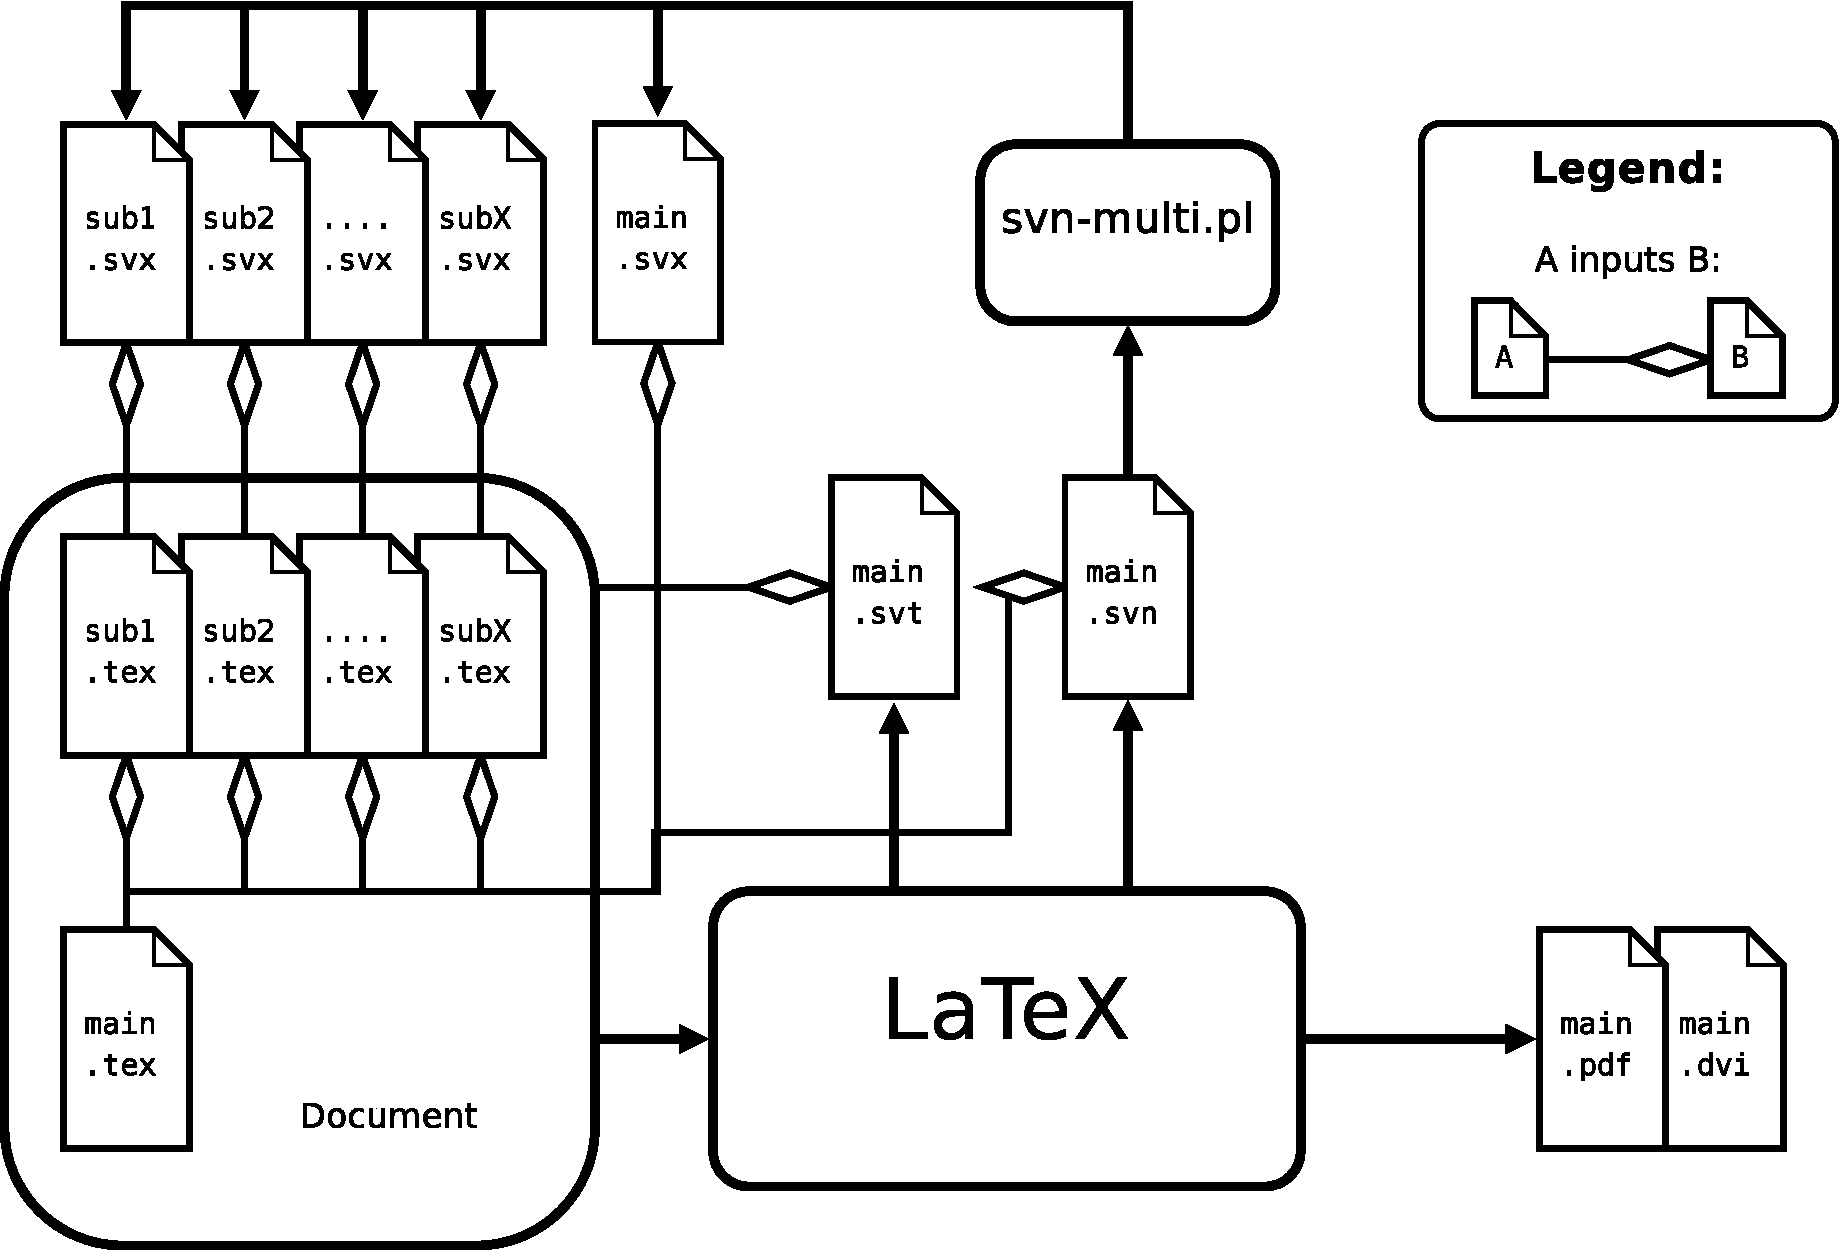
\includegraphics[width=.8\textwidth]{images/compilation.pdf}}
%   \caption{Compilation cycle of documents which use \svnmulti}\label{fig:compi}
% \end{figure}
% \fi
%
% \section{Known Issues}\label{sec:issues}
% This section lists some known issues of the \svnmulti package and tries to
% provide some workaround. Please feel free to write \svnmulti author if you
% detect any side effects or other issues causes by this package.
%
% \subsection{Packet \texttt{listings} uses \cs{input}}
% \textbf{Update:} Newer versions of \svnmulti avoid this issue by changing the catcodes
% back to normal while reading the |.svx| file.
% If a file \meta{basename}.\meta{extension} is typeset verbatim using
% |\lstinputlisting|, which uses |\input| to read the file, an existing
% \meta{basename}|.svx| file is also included as part of the listing. This can
% be avoided by code like this:
% \begin{verbatim}
%  {\makeatletter\let\input\@input
%  \lstinputlisting[options]{filename}
%  }
% \end{verbatim}
%
% \section{Package Dependencies and Acknowledgements}\label{sec:depack}
% This package uses some features from other packages and/or patches some macros
% of them to provide additional related features. This section is used to list
% this packages, their internal macro which got used and acknowledge the
% authors/maintainers of them. Please send error reports to the author of
% \svnmulti and not to the people listed below.\par
% All packages (including \svnmulti) stand under the \LaTeX\ Project Public
% Licence (LPPL) which can be found at
% \hbox{\url{http://www.latex-project.org/lppl/}} and can be freely downloaded
% from the Comprehensive TeX Archive Network (CTAN) at
% \hbox{\url{http://www.ctan.org/}}.
%
% \newenvironment*{DepPackage}[1]{\ignorespaces
% \subsection*{\pkg{#1}}%
% \def\thedeppackage{#1}%
% \def\infoline##1{\par\smallskip\textbf{##1}\hspace{1em}}%
% }
% {\infoline{Location:} CTAN: \url%
% {http://tug.ctan.org/pkg/\thedeppackage}}
%
% \begin{DepPackage}{hyperref}
% The macro \cs{svnnolinkurl} is resembling the \pkg{hyperref} macro
% |\nolinkurl| and uses some its internal macros from the |\url| macro
% definition.
% \infoline{Used internal macros:} |\hyper@normalise|, |\Hurl|
% \infoline{Version used:} 2008/11/18 v6.78m
% \infoline{Licence:} LPPL, any version
% \infoline{Authors/Maintainers:} Sebastian Rahtz, Heiko Oberdiek
% \end{DepPackage}
%
% \begin{DepPackage}{fink}
% The FiNK (File Name Keeper) package is used to get the file name and path of
% the input files. Two macros are patched to install hooks to execute own macros
% before and after each input file. This is only done if needed for an enabled
% option and therefore can be disabled using the option \op{old}.
% \infoline{Used internal macros:} |\fink@file|, |\fink@nextdir|,
% |\fink@nextext|, |\fink@nextbase|
% \infoline{Patched internal macros:} |\fink@prepare|, |\fink@restore|
% \infoline{Version used:} 2008/02/27 v2.1.1
% \infoline{Licence:} LPPL, any version
% \infoline{Author/Maintainer:} Didier Verna
% \end{DepPackage}
%
% \begin{DepPackage}{graphics}
% If the \op{graphics} option is enabled the following macro is patched to
% record the file name and path of the included graphic.
% \infoline{Patched internal macros:} |\Gin@setfile|
% \infoline{Version used:} 2006/02/20 v1.0o
% \infoline{Licence:} LPPL, any version
% \infoline{Author/Maintainer:} David Carlisle, \LaTeX3 Project
% \end{DepPackage}
%
% \begin{DepPackage}{pgf}
% Like the \pkg{graphics} package above a macro of this package is pathed to
% record the file names and paths of included images when the option
% \op{pgfimages} is enabled. Because this images pre-declares images for later
% use the internal declared `image macros' are patched as well.
% \infoline{Patched internal macros:} |\pgf@declareimage|,
% \hbox{|\pgf@image@|\meta{image name}|!|}
% \infoline{Used internal macros:} |\pgf@filename|, |\pgf@image|
% \infoline{Version used:} 2008/01/15 v2.00
% \infoline{Licence:} LPPL v1.3c and GPL v2
% \infoline{Author\&Maintainer:} Till Tantau
% \end{DepPackage}
%
% \begin{DepPackage}{latex}
% Parts of the macro definitions of the |\tableofcontents| macros from the
% |article| and |book| class of standard \LaTeX\ were used to define a similar
% \csi{tableofrevisions} macro for both this classes and other similar classes.
% \infoline{Version used:} 2005/09/16 v1.4f
% \infoline{Licence:} LPPL v1.3c
% \infoline{Authors/Maintainers:} \LaTeX3 Project
% \end{DepPackage}
%
%
% \section{Further Reading}
% The \textsf{svn-multi} package (in version 1.3) and its usage got discussed in
% the following articles:
%
% \begin{itemize}
%  \item[{[1]}] Martin Scharrer, ``Version Control of LaTeX Documents with
%  svn-multi'', The Prac\TeX\ Journal, (3), 2007.
%  URL: \url{http://www.tug.org/pracjourn/2007-3/scharrer/}
%  \item[{[2]}] Mark Eli Kalderon, ``LaTeX and Subversion'',
%  The Prac\TeX\ Journal, (3), 2007.
%  URL: \url{http://www.tug.org/pracjourn/2007-3/kalderon-svnmulti/}
%  \item[{[3]}] Uwe Ziegenhagen , ``LaTeX Document Management with Subversion'',
%  The Prac\TeX\ Journal, (3), 2007.
%  URL: \url{http://www.tug.org/pracjourn/2007-3/ziegenhagen/}
% \end{itemize}
%
% \StopEventually{}
% %%%%%%%%%%%%%%%%%%%%%%%%%%%%%%%%%%%%%%%%%%%%%%%%%%%%%%%%%%%%%%%%%%%%%%%%%%%%
% \section{Implementation}
% \subsection{Package Header}
% \subsubsection*{Package Identification}
%    \begin{macrocode}
\NeedsTeXFormat{LaTeX2e}[1999/12/01]
\ProvidesPackageSVN
  {$Id$}
  [\svnmulti@version\space SVN Keywords for multi-file LaTeX documents]
%    \end{macrocode}

% \subsubsection*{Options}
% Declaration of options and internal switches.
%    \begin{macrocode}
\RequirePackage{kvoptions}

\SetupKeyvalOptions{%
  family = svn-multi,
  prefix = @svnmulti@
}
\newif\if@svnmulti@anygraphic
\newif\if@svnmulti@autoload
\newif\if@svnmulti@autokw
\newif\if@svnmulti@autokwall

\DeclareVoidOption{old}{%
  \@svnmulti@verbatimtrue
  \@svnmulti@groupsfalse
  \@svnmulti@externalfalse
  \@svnmulti@graphicsfalse
  \@svnmulti@pgfimagesfalse
  \@svnmulti@autoloadfalse
  \@svnmulti@tablefalse
  \@svnmulti@filehooksfalse
  \@svnmulti@subgroupsfalse
}
\DeclareVoidOption{all}{%
  \@svnmulti@verbatimtrue
  \@svnmulti@groupstrue
  \@svnmulti@externaltrue
  \@svnmulti@graphicstrue
  \@svnmulti@pgfimagestrue
  \@svnmulti@autoloadtrue
  \@svnmulti@tabletrue
  \@svnmulti@filehookstrue
  \@svnmulti@subgroupstrue
}
\DeclareBoolOption[true]{verbatim}
\DeclareBoolOption[false]{groups}
\DeclareBoolOption[false]{external}
\DeclareBoolOption[false]{subgroups}
\DeclareBoolOption[false]{graphics}
\DeclareBoolOption[false]{pgfimages}
\DeclareStringOption{autoload}[true]
\DeclareBoolOption[false]{table}
\DeclareBoolOption[false]{filehooks}
\DeclareStringOption[false]{autokw}[all]

\ExecuteOptions{old}
\ProcessKeyvalOptions{svn-multi}
%    \end{macrocode}
%
% Enable dependent options:
%    \begin{macrocode}
\def\svn@depoption#1{%
  \csname if@svnmulti@#1\endcsname\else
  \message{svn-multi: Required option '#1' enabled.}%
  \csname @svnmulti@#1true\endcsname
  \fi
}

\if@svnmulti@groups
  \svn@depoption{filehooks}
\fi
\if@svnmulti@external
  \svn@depoption{filehooks}
\fi
\if@svnmulti@subgroups
  \svn@depoption{groups}
  \svn@depoption{filehooks}
\fi
\if@svnmulti@graphics
  \svn@depoption{external}
  \svn@depoption{autoload}
  \svn@depoption{filehooks}
\fi
\if@svnmulti@pgfimages
  \svn@depoption{external}
  \svn@depoption{autoload}
  \svn@depoption{filehooks}
\fi
\if@svnmulti@autoload
  \svn@depoption{external}
  \svn@depoption{filehooks}
\fi
\if@svnmulti@table
  \svn@depoption{groups}
  \svn@depoption{filehooks}
\fi
%    \end{macrocode}
%
% Check if \op{autoload} was set explicitly and obey the value.
%    \begin{macrocode}
\ifx\@svnmulti@autoload\@undefined
\else
\ifx\@svnmulti@autoload\empty
\else
\def\svn@temp{true}
\ifx\@svnmulti@autoload\svn@temp
  \@svnmulti@autoloadtrue
  \svn@depoption{external}
  \svn@depoption{filehooks}
\else
\def\svn@temp{false}
\ifx\@svnmulti@autoload\svn@temp
  \if@svnmulti@autoload
  \PackageWarning{svn-multi}{Option 'autoload' disabled.}
  \fi
  \@svnmulti@autoloadfalse
\else
  \PackageError{svn-multi}%
    {Invalid value for 'autoload' option: '\@svnmulti@autoload'^^J%
     ! Only 'true','false' or empty (='true') are allowed!}
\fi\fi\fi\fi
%    \end{macrocode}

% Set \op{autokw} modes:
%    \begin{macrocode}
\def\svn@temp{true}
\ifx\@svnmulti@autokw\svn@temp
  \@svnmulti@autokwtrue
  \@svnmulti@autokwalltrue
  \svn@depoption{filehooks}
\fi
\def\svn@temp{all}
\ifx\@svnmulti@autokw\svn@temp
  \@svnmulti@autokwtrue
  \@svnmulti@autokwalltrue
  \svn@depoption{filehooks}
\fi
\def\svn@temp{ext}
\ifx\@svnmulti@autokw\svn@temp
  \@svnmulti@autokwtrue
  \@svnmulti@autokwallfalse
\fi
\def\svn@temp{false}
\ifx\@svnmulti@autokw\svn@temp
  \@svnmulti@autokwfalse
  \@svnmulti@autokwallfalse
\fi
%    \end{macrocode}

% General switch if any graphic option is enabled:
%    \begin{macrocode}
\if@svnmulti@graphics
  \@svnmulti@anygraphictrue
\fi
\if@svnmulti@pgfimages
  \@svnmulti@anygraphictrue
\fi
%    \end{macrocode}
%

% \subsection{General Internal Macros}
% Some internal used macro which don't fit in any other section.
%
% \begin{macro}{\svn@ifempty}[1]{string}
% Tests if the given argument is empty. If so the first of the next two token
% will be expanded, the second one otherwise.
%    \begin{macrocode}
\def\svn@ifempty#1{%
  \begingroup
  \edef\svn@temp{#1}%
  \ifx\svn@temp\empty
    \endgroup
    \expandafter
    \@firstoftwo
  \else
    \endgroup
    \expandafter
    \@secondoftwo
  \fi
}
%    \end{macrocode}
% \end{macro}

% \begin{macro}{\svn@ifequal}[2]{string a}{string b}
% Tests if the given arguments are identical, \eg same strings. If so the first
% of the next two token will be expanded, the second one otherwise.
%    \begin{macrocode}
\def\svn@ifequal#1#2{%
  \begingroup
  \edef\svn@stringa{#1}%
  \edef\svn@stringb{#2}%
  \ifx\svn@stringa\svn@stringb
    \endgroup
    \expandafter
    \@firstoftwo
  \else
    \endgroup
    \expandafter
    \@secondoftwo
  \fi
}
%    \end{macrocode}
% \end{macro}

% \begin{macro}{\svn@ifvalidrev}[1]{macro name}
% Checks if the given macro (by name) is a valid revision, \ie defined and
% not equal to the init value.
%    \begin{macrocode}
\def\svn@ifvalidrev#1{%
  \begingroup
  \@ifundefined{#1}%
    {\let\svn@temp\svn@revinit}%
    {\expandafter\edef
     \expandafter\svn@temp\expandafter{\csname #1\endcsname}}%
  \ifnum\svn@temp=\svn@revinit\relax
    \endgroup
    \expandafter
    \@secondoftwo
  \else
    \endgroup
    \expandafter
    \@firstoftwo
  \fi
}
%    \end{macrocode}
% \end{macro}

% \begin{macro}{\svn@ifeof}[1]{input file handle}
% Checks if the input file is at the end-of-file (or not open).
%    \begin{macrocode}
\def\svn@ifeof#1{%
  \ifeof#1%
    \expandafter\@firstoftwo
  \else
    \expandafter\@secondoftwo
  \fi
}
%    \end{macrocode}
% \end{macro}

% \begin{macro}{\svn@ifonlyone}[1]{group name}
% Checks if there is only one element in the given group file list.
% It looks whether there is a comma in the list.
%    \begin{macrocode}
\def\svn@ifonlyone#1{%
  \expandafter\expandafter\expandafter
  \svn@@ifonlyone\csname @svng@#1@files\endcsname,\relax
}

\def\svn@@ifonlyone#1,#2\relax{%
  \svn@ifempty{#2}
}
%    \end{macrocode}
% \end{macro}

% \begin{macro}{\svn@input}[1]{file name/path}
% Macro to load |.svx| and |.svt| files.  The current keyword group is saved
% away and restored after the |.svx| file is loaded.  The macros |\IfFileExists|
% with |\@@input| are used because |\InputIfFileExists| got redefined by the
% \pkg{fink} package and there is no need to use \pkg{fink} for this files.
%    \begin{macrocode}
\def\svn@input#1{%
  \begingroup
    \let\svn@rg\svn@g
    \IfFileExists{#1}{\@@input #1\relax}{}%
    \global\let\svn@g\svn@rg
  \endgroup
}
%    \end{macrocode}
% \end{macro}

% \begin{macro}{\svn@inputsvx}[1]{file name/path without extension}
% Used to save and restore file keywords when reading |.svx| files.
% The normal catcodes are restored to avoid issues in special situations
% regarding input of verbatim files
% (e.g.\ \cs{lstinputlisting} from the \pkg{listings} package) or other
% cases where catcodes might have changes (e.g.\ `|%|' in |.dtx| files).
%    \begin{macrocode}
\def\svn@inputsvx#1{%
  \svn@pushfilestack
  \begingroup
  \svn@normalcatcodes
  \svn@input{#1.svx}%
  \endgroup
  \svn@popfilestack
}
%    \end{macrocode}
% \end{macro}

% \begin{macro}{\svn@normalcatcodes}
% Sets the default catcodes.
%    \begin{macrocode}
\def\svn@normalcatcodes{%
  \catcode`\\=0\relax
  \catcode`\{=1\relax
  \catcode`\}=2\relax
  \catcode`\$=3\relax
  \catcode`\&=4\relax
  \catcode`\^^M=5\relax
  \catcode`\#=6\relax
  \catcode`\^=7\relax
  \catcode`\_=8\relax
  \catcode`\ =10\relax
  \catcode`\@=12\relax
  \catcode`\~=13\relax
  \catcode`\%=14\relax
}
%    \end{macrocode}
% \end{macro}

% \subsection{Definition of init values}
% Initialisation of at least the revision to a numeric value is necessary to not
% break the |\ifnum| tests later in this package. The revision is initialised to
% -2, but will be set to 0 if an unexpanded |$||Rev:$| keyword is read. This way
% it can be tested if a file had any keyword macros or not.\par
% Note that there a two different macros for the document global keywords:\par
% The user level |\svn|\meta{kw} macros hold the global value and are only valid
% after a \LaTeX\ run. They are initialised here and defined in the |.svn|
% file which is read at the end of the package if it exists and written at the
% end of the document.\par
% The internal macros |\@svn@|\meta{kw} store the oldest (i.e. highest revision)
% keywords read so far from the \cs{svnid} and \cs{svnidlong} macros. They
% change during the document and are used to produce the values of the
% |\svn|\meta{kw} macros when the |.svn| file is written.\par
% Group wide macros are initialised when the group is first defined and have
% three different macros: |\svng@|\meta{group}|@|\meta{kw} (defined in |.svn|),
% |\@svng@|\meta{group}|@|\meta{kw} (accumulator) and also an access
% macro |\svncg|\meta{group} which uses
% |\svn@g|\meta{current group}|@|\meta{kw}.
%    \begin{macrocode}
% Init values
\def\svn@revinit{-2}
\let\svnrev\svn@revinit     \let\@svn@rev\svn@revinit
\let\ifsvnmodified\@secondoftwo
\def\@svn@modified{@secondoftwo}%
\def\svndate{}              \def\@svn@date{}
\def\svnauthor{}            \def\@svn@author{}
\def\svnyear{0000}          \def\@svn@year{0000}
\def\svnmonth{00}           \def\@svn@month{00}
\def\svnday{00}             \def\@svn@day{00}
\def\svnhour{00}            \def\@svn@hour{00}
\def\svnminute{00}          \def\@svn@minute{00}
\def\svnsecond{00}          \def\@svn@second{00}
\def\svntimezonehour{+00}   \def\@svn@timezonehour{+00}
\def\svntimezoneminute{00}  \def\@svn@timezoneminute{00}
\def\svnmainurl{NOT SET}    \def\svnmainfilename{NOT SET}
\def\svnurl{} \def\svnfname{}
\def\svn@temp{}

\def\svn@pg{} \def\svn@g{} \def\svn@cg{\svn@g} \def\svn@rg{\svn@pg}
\let\@svng@@files\relax

\def\svn@initfile{%
  \global\let\svnfilerev\svn@revinit
  \global\let\ifsvnfilemodified\@secondoftwo
  \gdef\svnfiledate{}%
  \gdef\svnfileauthor{}%
  \gdef\svnfileyear{0000}%
  \gdef\svnfilemonth{00}%
  \gdef\svnfileday{00}%
  \gdef\svnfilehour{00}%
  \gdef\svnfileminute{00}%
  \gdef\svnfilesecond{00}%
  \gdef\svnfiletimezonehour{+00}%
  \gdef\svnfiletimezoneminute{00}%
  \gdef\svnfileurl{}%
  \gdef\svnfilefname{}%
  \gdef\svnfiledir{}%
}
\svn@initfile

\newif\ifsvn@modified
%    \end{macrocode}

% \subsection{Auto-Keywords}

% Special care must be taken for the line feed character, otherwise it causes an 
% error if \op{autokw} is disabled.
%    \begin{macrocode}
\begingroup
\@makeother\^^L
\if@svnmulti@autokw
\gdef\svne@ff{^^L}
\fi
\endgroup
%    \end{macrocode}

%    \begin{macrocode}
\if@svnmulti@autokw
%    \end{macrocode}
% 
%    \begin{macrocode}
\newread\svne@read
%    \end{macrocode}

% \begin{macro}{\svne@catcodes}
% Sets the catcodes for verbatim input reading. Also removes the end-of-line 
% character.
% \begin{macrocode}
\newcommand*{\svne@catcodes}{%
  \let\do\@makeother
  \endlinechar=-1%
  \dospecials
  \do\-\do\:\do\.\do\^^L%
}
%    \end{macrocode}
% \end{macro}

% \begin{macro}{\svne@readline}[1]{macro}
% Reads the next line to the provided macro and handles the end-of-file case 
% correctly.
%    \begin{macrocode}
\def\svne@readline#1{%
  \ifeof\svne@read
    \def#1{}%
  \else
    \read\svne@read to #1\relax
  \fi
}
%    \end{macrocode}
% \end{macro}

% \begin{macro}{\svne@gobblerest}
% Gobbles the rest of the current entry.
%    \begin{macrocode}
\def\svne@gobblerest{%
  \ifeof\svne@read
    \let\next\relax
  \else
    \read\svne@read to \svn@temp
    \ifx\svn@temp\svne@ff
      \let\next\relax
    \else
      \let\next\svne@gobblerest
    \fi
  \fi
  \next
}
%    \end{macrocode}
% \end{macro}

% \begin{macro}{\svne@endread}
% Stops the reading process of the entries file.
%    \begin{macrocode}
\def\svne@endread{%
  \closein\svne@read
}
%    \end{macrocode}
% \end{macro}

% \begin{macro}{\svne@parseentriesfile}[1]{file path}
%    \begin{macrocode}
\newcommand*{\svne@parseentriesfile}[1]{%
  \begingroup
    \let\next\relax
%    \end{macrocode}
% Open the format file to read the version number. If this file does not exists
% (true for recent svn versions) a valid default value is used and the true
% version number is read from the |entries| file.
%    \begin{macrocode}
    \def\svne@version{8}%
    \openin\svne@read=#1format\relax
    \ifeof\svne@read\else
      \svne@readline\svne@version
      \closein\svne@read
    \fi
%    \end{macrocode}
% Check the format version:
%    \begin{macrocode}
      \ifnum\svne@version>7\relax
%    \end{macrocode}
% Now open the entries file and read the version number from there again.
%    \begin{macrocode}
        \openin\svne@read=#1entries\relax
        \ifeof\svne@read\else
          \svne@catcodes
          \svne@readline\svne@version
%    \end{macrocode}
% Check the version and call the parse macros if OK:
%    \begin{macrocode}
          \ifnum\svne@version>7\relax
            \def\next{\svne@parsedirentry
                      \svne@parseentries}%
          \else
            \closein\svne@read
          \fi
        \fi
      \fi
    \next
  \endgroup
}
%    \end{macrocode}
% \end{macro}

% \begin{macro}{\svne@parsedirentry}
% Reads the first entry which is the directory entry and sets its URL as base 
% URL for all other entries.
% \begin{macrocode}
\newcommand*{\svne@parsedirentry}{%
  \svne@readline\svne@name
  \svne@readline\svne@kind
  \svn@ifempty{\svne@name}%
    {\svn@ifequal{\svne@kind}{dir}%
      {%
        {\svne@readline\svn@temp}%
        \svne@readline\svne@baseurl
        \svne@gobblerest
      }{}%
    }{}%
}
%    \end{macrocode}
% \end{macro}

% \begin{macro}{\svne@scandate}
% \begin{macro}{\svne@scandate@}
% Parses the date from the svn entries file. Special care is taken to handle the 
% case when the TeX parsing would fail. The catcode of the characters '|-|', 
% '|:|', '|.|' used inside the date is set explicitly to ensure the correct 
% value.
%
% \begin{macrocode}
\begingroup

\@makeother\-
\@makeother\:
\@makeother\.

\gdef\svne@scandate#1{%
  \expandafter\svne@scandate@#1\empty
  0000-00-00T00:00:00.00000Z\empty\empty
}

\gdef\svne@scandate@#1-#2-#3T#4:#5:#6.#7\empty#8\empty{%
  \xdef\svnfileyear{#1}%
  \gdef\svnfilemonth{#2}%
  \gdef\svnfileday{#3}%
  \gdef\svnfilehour{#4}%
  \gdef\svnfileminute{#5}%
  \gdef\svnfilesecond{#6}%
  \gdef\svnfiletimezonehour{+00}%
  \gdef\svnfiletimezoneminute{00}%
  \gdef\svnfiledate{#1-#2-#3 #4:#5:#6Z}%
  \def\svne@date{#1-#2-#3 #4:#5:#6Z}%
}

\endgroup
%    \end{macrocode}
% \end{macro}
% \end{macro}

% \begin{macro}{\svne@parseentries}
%    \begin{macrocode}
\newcommand*{\svne@parseentries}{%
  \svn@ifeof{\svne@read}%
  {}%
  {%
    \svne@readline\svne@name
    \@onelevel@sanitize\svne@name
    \svn@ifeof{\svne@read}%
    {}%
    {%
    \svne@readline\svne@kind
    \svn@ifequal{\svne@kind}{file}%
      {%
      \svne@readline\svn@temp
      \svne@readline\svn@temp
      \svne@readline\svn@temp
      \svne@readline\svn@temp
      \svne@readline\svn@temp
      \svne@readline\svn@temp
      \svne@readline\svne@date
      \svne@readline\svne@rev
      \svne@readline\svne@author
      %\@onelevel@sanitize\svne@date
      \svne@scandate{\svne@date}%
      \edef\svne@url{\svne@baseurl/\svne@name}%
      \svne@handleentry
      }{}%
    \svne@gobblerest
    \svne@parseentries
    }%
  }%
}
%    \end{macrocode}
% \end{macro}

% \begin{macro}{\svne@handleentry}
% This macro is called for every entry except the first one which stands for the 
% directory. The VC data is located in the following macros: \csi{svne@name}, 
% \csi{svne@date}, \csi{svne@rev}, \csi{svne@author}, \csi{svne@url}.
%
% This implementation sets the correct keywords and calls the update macro to 
% emulate the behaviour of \cs{svnidlong}. Then the \cs{svne@endread} macro is 
% used to stop the file reading.
%    \begin{macrocode}
\def\svne@handleentry{%
  \ifx\svne@rev\empty
    \let\svne@rev\svn@revinit
  \fi
  \svn@ifequal{\svne@name}{\svnfilefname}%
    {%
      \message{^^J%
        Read from '.svn/entries' file:^^J%
        Filename:  \svne@name^^J%
        Date:      \svne@date^^J%
        Revision:  \svne@rev^^J%
        Author:    \svne@author^^J%
        HeadURL:   \svne@url^^J%
        ^^J%
      }%
      \svnkwdef{Filename}{\svne@name}%
      \svnkwdef{Date}{\svne@date}%
      \svnkwdef{Revision}{\svne@rev}%
      \svnkwdef{Author}{\svne@author}%
      \svnkwdef{HeadURL}{\svne@url}%
      \@svn@updateid{\svne@rev}{\svne@date}{\svne@author}{\svne@url}%
      \svne@endread
    }{}%
}%
%    \end{macrocode}
% \end{macro}

% \begin{macro}{\svnegetfile}[1]{file path}
%    \begin{macrocode}
\def\svnegetfile#1{%
  \begingroup
    \svn@getfilename{#1}%
    \edef\svnfilefname{\svnfilefname}%
    \@onelevel@sanitize\svnfilefname
    \svne@parseentriesfile{\svnfiledir .svn/}%
    \svne@parseentriesfile{\svnfiledir _svn/}%
  \endgroup
}
%    \end{macrocode}
% \end{macro}

% Load keywords of main document at begin of the document body if option is set 
% to 'all'.
%    \begin{macrocode}
\if@svnmulti@autokwall
\AtBeginDocument{%
    \svnegetfile{\jobname.\svn@mainext}%
}
\fi
%    \end{macrocode}

%    \begin{macrocode}
\fi
%    \end{macrocode}


% \subsection{Timezone macros}
% \begin{macro}{\svntimezone}
% \begin{macro}{\svnfiletimezone}
% \begin{macro}{\svncgtimezone}
% These macros return the global, file-local and current group time zones,
% respectively. Since v1.4 the minute part is returned as well and the macro
% removes manually added |00| after it to support older documents.
% \changes{v1.4}{2009/02/27}{Return now full timezone (hour + minute part).
% Manually added 00 minutes are removed.}
%    \begin{macrocode}
\def\svntimezone{\svntimezonehour\svntimezoneminute\svn@gobblezeros}
\def\svnfiletimezone{\svnfiletimezonehour\svnfiletimezoneminute\svn@gobblezeros}
\def\svncgtimezone{\svncgtimezonehour\svncgtimezoneminute}
%    \end{macrocode}
% \end{macro}
% \end{macro}
% \end{macro}

% \begin{macro}{\svn@gobblezeros}
% \begin{macro}{\svn@gobblezeros@}
% This two cascaded macros remove a trailing |00| and are used by
% \cs{svnfiletimezone} and \cs{svntimezone}.
%    \begin{macrocode}
\def\svn@gobblezeros{%
  \futurelet\svn@nextchar\svn@gobblezeros@
}
\def\svn@gobblezeros@{%
  \let\@tempa=\relax
  \def\@tempb{0}%
  \ifx0\svn@nextchar
    \let\@tempa=\@gobbletwo
  \fi
  \@tempa
}
%    \end{macrocode}
% \end{macro}
% \end{macro}

% \begin{macro}{\svntime}
% \begin{macro}{\svnfiletime}
% \begin{macro}{\svncgtime}
% This macros simple use the hour, minute and second macros.
%    \begin{macrocode}
\def\svntime{\svnhour:\svnminute:\svnsecond}
\def\svnfiletime{\svnfilehour:\svnfileminute:\svnfilesecond}
\def\svncgtime{\svncghour:\svncgminute:\svncgsecond}
%    \end{macrocode}
% \end{macro}
% \end{macro}
% \end{macro}

% \subsection{\textit{Today} macros}
% These macros use the |\today| macro to typeset the current date using the
% local language settings. Thanks and credit goes to Manuel P\'egouri\'e-Gonnard
% for suggesting this feature and for providing the code.
% \begin{macro}{\svntoday}
%    \begin{macrocode}
\newcommand*{\svntoday}{%
  \begingroup
    \year\svnyear \month\svnmonth \day\svnday
    \relax \today
  \endgroup
}
%    \end{macrocode}
% \end{macro}
%
% \begin{macro}{\svnfiletoday}
%    \begin{macrocode}
\newcommand*{\svnfiletoday}{%
  \begingroup
    \year\svnfileyear \month\svnfilemonth \day\svnfileday
    \relax \today
  \endgroup
}
%    \end{macrocode}
% \end{macro}
%
% \begin{macro}{\svncgtoday}
%    \begin{macrocode}
\newcommand*{\svncgtoday}{%
  \@ifundefined{svng@\svn@cg @year}{??}{%
    \begingroup
      \year\svncgyear \month\svncgmonth \day\svncgday
      \relax \today
    \endgroup
  }%
}%
%    \end{macrocode}
% \end{macro}

% \subsection{Id macros}
% \subsubsection{Normal Id}
% \begin{macro}{\svnid}
% Calls \cs{svnkwsave} with |\@svnidswtrue| so that the Id keyword will be
% parsed at the end of \cs{svnkwsave}.
%    \begin{macrocode}
\newcommand*{\svnid}{%
  \@svnidswtrue
  \svnkwsave
}
\newif\if@svnidsw
\@svnidswfalse
%    \end{macrocode}
% \end{macro}
%

% \begin{macro}{\svn@scanId}[5]{file name}{revision}{date (YYYY-MM-DD)}{time
% (HH:MM:SSZ)}{author (username)}
% Scans svn Id (after it got parsed by \cs{svnkwsave}).  Awaits only Id value
% without leading `|Id:|' and a trailing |\relax| as end marker.  It calls
% \cs{@svn@scandate} to extract the date information and \cs{@svn@updateid} to
% update global Id values and also sets the appropriate keywords.
%    \begin{macrocode}
\def\svn@scanId#1 #2 #3 #4 #5\relax{%
  \@svn@scandate{#3 #4}%
  \@svn@updateid{#2}{#3 #4}{#5}{#1}%
  \svnkwdef{Filename}{#1}%
  \svnkwdef{Date}{#3 #4}%
  \svnkwdef{Revision}{#2}%
  \svnkwdef{Author}{#5}%
}
%    \end{macrocode}
% \end{macro}
%

% \begin{macro}{\@svn@updateid}[4]{rev}{date}{author (username)}{url}
% We first define the expanded arguments to variables for the user.  The
% expansion is needed because the arguments content is mostly generic like
% |\svn@value| which can change very soon after this macro.
%    \begin{macrocode}
\def\@svn@updateid#1#2#3#4{%
  \xdef\svnfilerev{#1}%
  \ifsvn@modified
    \global\let\ifsvnfilemodified\@firstoftwo
  \else
    \global\let\ifsvnfilemodified\@secondoftwo
  \fi
  \xdef\svnfiledate{#2}%
  \xdef\svnfileauthor{#3}%
  \xdef\svnfileurl{#4}%
  \svn@getfilename\svnfileurl%
%    \end{macrocode}
% Then we check if the revision is non-empty (not yet expanded by subversion?)
% and larger then the current maximum value |\@svn@rev|.  If yes we save all
% value to save them in the .svn-file later.
%    \begin{macrocode}
  \ifx\svnfilerev\empty\else
    \ifnum\@svn@rev<\svnfilerev
      \xdef\@svn@rev{\svnfilerev}%
      \xdef\@svn@modified{\ifsvnfilemodified{@firstoftwo}{@secondoftwo}}%
      \xdef\@svn@date{\svnfiledate}%
      \xdef\@svn@author{\svnfileauthor}%
      \xdef\@svn@year{\svnfileyear}%
      \xdef\@svn@month{\svnfilemonth}%
      \xdef\@svn@day{\svnfileday}%
      \xdef\@svn@hour{\svnfilehour}%
      \xdef\@svn@minute{\svnfileminute}%
      \xdef\@svn@second{\svnfilesecond}%
      \xdef\@svn@timezonehour{\svnfiletimezonehour}%
      \xdef\@svn@timezoneminute{\svnfiletimezoneminute}%
      \xdef\@svn@url{\svnfileurl}%
      \xdef\@svn@fname{\svnfilefname}%
    \fi

    \if@svnmulti@groups
      \ifx\svn@g\empty\else
        \svn@updategroup{\svn@g}%
      \fi
      \if@svnmulti@subgroups
        \ifsvnsubgroups
          \svn@updategroup{\svn@filedir\svn@filebase}%
        \fi
      \fi
    \fi
  \fi
}

\def\@svncg@save#1#2{%
  \expandafter\xdef\csname @svng@\svn@g @#1\endcsname{#2}%
}

%    \end{macrocode}
% \end{macro}
%

% \subsubsection{Long Id}
% \begin{macro}{\svnidlong}
% We clear the keyword value first to reduce the risk though bad user input.
%    \begin{macrocode}
\newcommand{\svnidlong}{%
  \svnkwdef{URL}{}%
  \svnkwdef{Date}{}%
  \svnkwdef{Revision}{0}%
  \svnkwdef{Author}{}%
%    \end{macrocode}
% Read arguments verbatim or non-verbatim.
%    \begin{macrocode}
  \if@svnmulti@verbatim
    \expandafter\svnidlong@readverb
  \else
    \expandafter\svnidlong@readargs
  \fi
}
%    \end{macrocode}
% \end{macro}
%
% \begin{macro}{\svnidlong@readverb}
% The following macros read the four arguments of |\svnidlong| one-by-one with
% verbatim mode deactivated between them to ignore all comments. The macro 
% |\@ifnextchar| is used to get rid of all spaces (and therefore comments) between
% the arguments. An error message is printed if a wrong syntax is discovered.
%    \begin{macrocode}
\def\svnidlong@readverb{%
  \@ifnextchar\bgroup
    {\svnidlong@readverb@\svnidlong@readverb@a}%
    {\PackageError{svn-multi}{Wrong syntax for \string\svnidlong}{}}%
}
%    \end{macrocode}
% Sets up verbatim mode and calls the macro given as an argument.
%    \begin{macrocode}
\def\svnidlong@readverb@#1{%
  \begingroup
  \svn@catcodes
  \catcode`\{=1\relax
  \catcode`\}=2\relax
  #1%
}
%    \end{macrocode}
% Reads first argument, ignores spaces and comments and calls next macro.
%    \begin{macrocode}
\def\svnidlong@readverb@a#1{%
  \endgroup
  \svnkwsave@read #1\relax
  \@ifnextchar\bgroup
    {\svnidlong@readverb@\svnidlong@readverb@b}%
    {\PackageError{svn-multi}{Wrong syntax for \string\svnidlong}{}}%
}
%    \end{macrocode}
% Reads second argument, ignores spaces and comments and calls next macro.
%    \begin{macrocode}
\def\svnidlong@readverb@b#1{%
  \endgroup
  \svnkwsave@read #1\relax
  \@ifnextchar\bgroup
    {\svnidlong@readverb@\svnidlong@readverb@c}%
    {\PackageError{svn-multi}{Wrong syntax for \string\svnidlong}{}}%
}
%    \end{macrocode}
% Reads third argument, ignores spaces and comments and calls next macro.
%    \begin{macrocode}
\def\svnidlong@readverb@c#1{%
  \endgroup
  \svnkwsave@read #1\relax
  \@ifnextchar\bgroup
    {\svnidlong@readverb@\svnidlong@readverb@d}%
    {\PackageError{svn-multi}{Wrong syntax for \string\svnidlong}{}}%
}
%    \end{macrocode}
% Reads last argument, scans date if not empty and calls the Id update macro.
%    \begin{macrocode}
\def\svnidlong@readverb@d#1{%
  \endgroup
  \svnkwsave@read #1\relax
  \ifx\svnkwDate\empty\else
    \@svn@scanlongdate{\svnkwDate}%
  \fi
  \@svn@updateid{\svnkw{Revision}}{\svnkw{Date}}%
  {\svnkw{Author}}{\svnkw{URL}}%
  \ignorespaces
}
%    \end{macrocode}
% \end{macro}

% \begin{macro}{\svn@catcodes}
% Changes all \TeX-special character to category ``other''. The newline aka
% return is changed to category ``ignore'' so line breaks are not taken as part
% of the verbatim arguments.
%    \begin{macrocode}
\if@svnmulti@verbatim
\def\svn@catcodes{%
  \let\do\@makeother
  \dospecials
  \catcode`\^^M9
  \catcode`\ 10
  \catcode`\{1
  \catcode`\}2
}
\else
  \def\svn@catcodes{}
\fi
%    \end{macrocode}
% \end{macro}
%
% \begin{macro}{\svnidlong@readargs}[4]{Keyword 1}{Keyword 2}{Keyword 3}
% {Keyword 4}
% Calls sub macro for all four arguments and ends the catcode changes made
% by \cs{svnidlong}.
%    \begin{macrocode}
\def\svnidlong@readargs#1#2#3#4{%
    \svnkwsave@read #1\relax
    \svnkwsave@read #2\relax
    \svnkwsave@read #3\relax
    \svnkwsave@read #4\relax
  \endgroup
%    \end{macrocode}
% Now the update macros for date and id are called.
%    \begin{macrocode}
  \ifx\svnkwDate\empty\else
    \@svn@scanlongdate{\svnkwDate}%
  \fi
  \@svn@updateid{\svnkw{Revision}}{\svnkw{Date}}%
  {\svnkw{Author}}{\svnkw{URL}}%
  \ignorespaces
}%
%    \end{macrocode}
% \end{macro}

% \subsection{KeyWord Macros}
% \begin{macro}{\svnkwsave}
% Enabled verbatim mode and uses a sub macro to read the arguments afterwards.
%    \begin{macrocode}
\def\svnkwsave{%
  \begingroup
    \svn@catcodes
    \svnkwsave@readargs
}
%    \end{macrocode}
% \end{macro}

% \begin{macro}{\svnkwsave@readargs}[1]{\$kw: value\$}
% Reads full argument, calls parse submacro and ends catcode changes.
% If \cs{svnkwsave} was called by \cs{svnid} scans the id keyword by calling the
% scan macro.
%    \begin{macrocode}
\gdef\svnkwsave@readargs#1{%
    \svnkwsave@read#1\relax
  \endgroup
  \if@svnidsw
    \ifx\svnkwId\empty\else
      \expandafter
      \svn@scanId\svnkwId\relax
      \@svnidswfalse
    \fi
  \fi
  \ignorespaces
}
%    \end{macrocode}
% \end{macro}

% \begin{macro}{\svnkwsave@read}[1]{keyword line without surrounding \$ \$}
% Reads the full keyword and strips the dollars.
%    \begin{macrocode}
\begingroup
\if@svnmulti@verbatim
\catcode`\$=12
\fi
\gdef\svnkwsave@read $#1$\relax{%
  \svn@checkcolon#1:\relax
}
\endgroup
%    \end{macrocode}
% \end{macro}

% \begin{macro}{\svnkwsave@parse}[2]{key}{value}
% Parse the keyword and save it away.
%    \begin{macrocode}
\begingroup
\catcode`\$=11
\gdef\svnkwsave@parse$#1:#2${%
  \expandafter\xdef\csname svnkw#1\endcsname{#2}%
}%
\endgroup
%    \end{macrocode}
% \end{macro}

% \begin{macro}{\svnkwdef}[2]{key}{value}
% First we check if there is a `setter'-macro for the keyword called
% \cs{svnkwdef@}\meta{keyword}.
%    \begin{macrocode}
\newcommand{\svnkwdef}[2]{%
  \@ifundefined{svnkwdef@#1}%
%    \end{macrocode}
% If not we call the general macro \cs{svnkwdef@}.
%    \begin{macrocode}
    {\svnkwdef@{#1}{#2}}%
%    \end{macrocode}
% If yes we just call it with the value as argument.
%    \begin{macrocode}
    {\csname svnkwdef@#1\endcsname{#2}}%
}
%    \end{macrocode}
% \end{macro}

% \begin{macro}{\svnkwdef@}[2]{key}{value}
% This macro defines the second argument under \cs{svnkw}\meta{1st argument}.
% The |\xdef| is used to expand the content first (needed for internal use) and
% make the definition globally.
%    \begin{macrocode}
\newcommand{\svnkwdef@}[2]{%
  \expandafter\xdef\csname svnkw#1\endcsname{#2}%
}
%    \end{macrocode}
% Example: |\svnkwdef{Revision}{23}| will define |\svnkwRevision| as 23.
% \end{macro}

% \begin{macro}{\svnkwdef@Rev}
% \begin{macro}{\svnkwdef@Author}
% \begin{macro}{\svnkwdef@Date}
% \begin{macro}{\svnkwdef@URL}[1]{value}
% `Setter'-macros for single keywords, used by \cs{svnkwdef}.\\ These are needed
% to have have a common value for all alternative keyword names ala |Rev|,
% |Revision|, |LastChangedRevision|.
%
% The keywords |Author| and |Date| are just calling \cs{svnkwdef@} with a fixed
% first argument.  For the revision the value is checked if empty and then a 0
% is substituted. Also a temp counter is used to strip any trailing characters 
% like `M' which indicate an exported and modified file.
%    \begin{macrocode}
\def\svnkwdef@Rev#1{%
  \svn@ifempty{#1}%
    {\svnkwdef@{Rev}{0}}%
    {%
     \afterassignment\svnkwdef@Rev@
     \@tempcnta=#1\relax
    }%
}
\def\svnkwdef@Rev@#1\relax{%
  \svnkwdef@{Rev}{\the\@tempcnta}%
  \def\svn@temp{#1}%
  \if M\svn@temp\relax
    \global\svn@modifiedtrue
  \else
    \if *\svn@temp\relax
      \global\svn@modifiedtrue
    \else
      \global\svn@modifiedfalse
    \fi
  \fi
}
\def\svnkwdef@Author#1{\svnkwdef@{Author}{#1}}
\def\svnkwdef@Date#1{\svnkwdef@{Date}{#1}}
\def\svnkwdef@URL#1{\svnkwdef@{HeadURL}{#1}}
%    \end{macrocode}
% The long keywords are defined then as aliases of the short,\\
% first for writing
%    \begin{macrocode}
\let\svnkwdef@Revision=\svnkwdef@Rev
\let\svnkwdef@LastChangedRevision=\svnkwdef@Rev
\let\svnkwdef@LastChangedBy=\svnkwdef@Author
\let\svnkwdef@LastChangedDate=\svnkwdef@Date
%    \end{macrocode}
% and then for reading.
%    \begin{macrocode}
\def\svnkwRevision{\svnkwRev}
\def\svnkwLastChangedRevision{\svnkwRev}
\def\svnkwLastChangedBy{\svnkwAuthor}
\def\svnkwLastChangedDate{\svnkwDate}
\def\svnkwURL{\svnkwHeadURL}
%    \end{macrocode}
% So \eg |\svnkw{LastChangedRevision}| is always be the
% same as |\svnkw{Rev}|.
% \end{macro}
% \end{macro}
% \end{macro}
% \end{macro}

% We define default values for normal keywords. Keyword |Filename| is the name
% given by |Id| and not a real keyword.
%    \begin{macrocode}
\svnkwdef{Rev}{0}
\svnkwdef{Date}{}
\svnkwdef{Author}{}
\svnkwdef{Filename}{}
\svnkwdef{HeadURL}{}
%    \end{macrocode}

% \begin{macro}{\svnkw}[1]{keyword name}
% Macro to get keyword value. Just calls \cs{svnkw}\meta{ARGUMENT} where
% the argument interpreted as text. So \eg |\svnkw{Date}| is the same as
% |svnkwDate| but this could be changed later so always use this interface
% to get the keyword values.
%
% \changes{v1.2}{2007/06/22}{Added warning when a wrong, maybe
% misspelled, keyword is given.}
%    \begin{macrocode}
\newcommand{\svnkw}[1]{%
  \@ifundefined{svnkw#1}%
    {\PackageWarning{svn-multi}{SVN keyword '#1' not defined (typo?)}}%
    {\csname svnkw#1\endcsname}%
}%
%    \end{macrocode}
% \end{macro}
%

% \subsection{Keyword check and strip macros}
% The following macros are used to test whether the given keywords are fully
% expanded or not.
% Subversion supports unexpanded keywords as input with or without colon and
% with or without trailing space(s), \ie a:~|$KW$|, b:~|$KW:$| or c:~|$KW: $|.
% To avoid \LaTeX{} syntax errors in this pre-commit state the keyword is
% checked by the following macros. Unexpanded keywords result in an empty value.
% Also leading and trailing spaces are removed.
%
% \begin{macro}{\svn@checkcolon}[2]{key}{potential value, might be empty}
% Checks if the keyword contains a colon. It is called by \cs{svnkwsave@read}
% with a trailing |:\relax| so that \#2 will be empty if there is no earlier
% colon or will hold the value with this trailing colon otherwise.
% The first case means that the keyword is unexpanded without colon (case a)
% which leads to an empty value. In the second case \cs{svn@stripcolon} is
% called to strip the colon and surrounding spaces. The final value is
% returned by |\svn@value|.
%    \begin{macrocode}
\def\svn@checkcolon#1:#2\relax{%
  \svn@ifempty{#2}%
    {\svnkwdef{#1}{}}%
    {\svn@stripcolon#2\relax\svnkwdef{#1}{\svn@value}}%
}
%    \end{macrocode}
% \end{macro}

% \begin{macro}{\svn@stripcolon}[1]{potential value}
% Strips the previous added colon (for \cs{svn@checkcolon}).
% The remaining argument is checked if it's empty (case b) or only a space
% (case c). Otherwise the keyword is expanded and \cs{svn@stripspace} is
% called to strip the spaces.
%    \begin{macrocode}
\def\svn@stripcolon#1:\relax{%
  \svn@ifempty{#1}%
    {\gdef\svn@value{}}%
    {\svn@ifequal{#1}{ }%
      {\gdef\svn@value{}}%
      {\svn@stripspace#1\relax\relax}%
    }%
}
%    \end{macrocode}
% \end{macro}

% \begin{macro}{\svn@stripspace}[2]{first character}{rest of string}
% Strips leading space if present and calls \cs{svn@striptrailingspace} to
% strip the trailing space.
%    \begin{macrocode}
\def\svn@stripspace#1#2\relax{%
  \svn@ifequal{#1}{ }%
    {\gdef\svn@value{#2}}%
    {\svn@striptrailingspace#1#2\relax}%
}
%    \end{macrocode}
% \end{macro}

% \begin{macro}{\svn@striptrailingspace}[1]{string}
% Strips trailing space using the macros parameter text. Must be called with
% |\relax| as end marker.
%    \begin{macrocode}
\def\svn@striptrailingspace#1 \relax{%
  \gdef\svn@value{#1}%
}
%    \end{macrocode}
% \end{macro}

% \begin{macro}{\svn@gdefverb}[1]{macro}
%    \begin{macrocode}
\def\svn@gdefverb#1{%
  \begingroup
    \def\svn@temp{#1}%
    \begingroup
      \if@svnmulti@verbatim
        \svn@catcodes
      \fi
      \svn@gdefverb@
}
%    \end{macrocode}
% \end{macro}

% \begin{macro}{\svn@defverb@}[1]{verbatim stuff}
%    \begin{macrocode}
\def\svn@gdefverb@#1{%
    \endgroup
    \expandafter\gdef\svn@temp{#1}%
  \endgroup
}
%    \end{macrocode}
% \end{macro}

% \begin{macro}{\svn@namegdefverb}[1]{macro name}
%    \begin{macrocode}
\def\svn@namegdefverb#1{%
  \begingroup
    \expandafter\def
    \expandafter\svn@temp
    \expandafter{\csname #1\endcsname}%
    \begingroup
      \if@svnmulti@verbatim
        \svn@catcodes
      \fi
      \svn@gdefverb@
}
%    \end{macrocode}
% \end{macro}


% \subsection{Date Macros}
% \begin{macro}{\@svn@scandate}[1]{date}
% Scans data information in Id keyword and saves them in macros.
%    \begin{macrocode}
\def\@svn@scandate#1{\@svn@scandate@#1\relax}

\def\@svn@scandate@#1-#2-#3 #4:#5:#6#7#8\relax{%
  \gdef\svnfileyear{#1}%
  \gdef\svnfilemonth{#2}%
  \gdef\svnfileday{#3}%
  \gdef\svnfilehour{#4}%
  \gdef\svnfileminute{#5}%
  \gdef\svnfilesecond{#6#7}%
  \gdef\svnfiletimezonehour{+00}%
  \gdef\svnfiletimezoneminute{00}% #8 always 'Z' for Zulu-time (UTC)
}
%    \end{macrocode}
% \end{macro}

% \begin{macro}{\@svn@scanlongdate}[8]{Year}{Month}{Day}{Hour}{Minute}{Second}
% {Timezone}{Date description string (ignored)}
% Scans date information in Date keyword and saves them in macros.
%    \begin{macrocode}
\def\@svn@scanlongdate#1{\expandafter\@svn@scanlongdate@#1\relax}
%
\def\@svn@scanlongdate@#1-#2-#3 #4:#5:#6 #7 #8\relax{%
  \gdef\svnfileyear{#1}%
  \gdef\svnfilemonth{#2}%
  \gdef\svnfileday{#3}%
  \gdef\svnfilehour{#4}%
  \gdef\svnfileminute{#5}%
  \gdef\svnfilesecond{#6}%
  \@svn@parsetimezone#7\relax%
}
%    \end{macrocode}
% \end{macro}

% \begin{macro}{\@svn@parsetimezone}[5]{sign (+/-)}{hour first digit}{hour
% second digit}{minute first digit}{minute second digit}
% Scans timezone and splits hour and minute part.
%    \begin{macrocode}
\def\@svn@parsetimezone#1#2#3#4#5\relax{%
  \gdef\svnfiletimezonehour{#1#2#3}%
  \gdef\svnfiletimezoneminute{#4#5}%
}
%    \end{macrocode}
% \end{macro}

% \begin{macro}{\svnpdfdate}
% Returns date in a format needed for |\pdfinfo|.
%    \begin{macrocode}
\def\svnpdfdate{%
  \svnyear\svnmonth\svnday
  \svnhour\svnminute\svnsecond\svntimezonehour'\svntimezoneminute'%
}
%    \end{macrocode}
% \end{macro}

% \subsection{Mainfile Makros}
% \begin{macro}{\svnsetmainfile}
% Saves the current |HeadURL| and |Filename| keywords to macros.
% Will be called automatically in the preamble.
% \changes{v1.2}{2007/06/22}{New macro}
%    \begin{macrocode}
\newcommand{\svnsetmainfile}{%
  \xdef\svnmainurl{\svnfileurl}%
  \xdef\svnmainfilename{\svnfilefname}%
}
\AtBeginDocument{\svnsetmainfile}
%    \end{macrocode}
% \end{macro}

% \subsection{Register and FullName Macros}
% \begin{macro}{\svnRegisterAuthor}[2]{author username}{Full Name}
% Saves the author's name by defining |svn@author@|\meta{username} to it.
%    \begin{macrocode}
\newcommand{\svnRegisterAuthor}[2]{%
  \expandafter\def\csname svn@author@#1\endcsname{#2}%
}
%    \end{macrocode}
% \end{macro}

% \begin{macro}{\svnFullAuthor}
% \begin{macro}{\svnFullAuthor*}
% We test if the starred or the normal version is used and call the
% appropriate submacro |svnFullAuthor@star| or |svnFullAuthor@normal|.
% \changes{v1.2}{2007/06/22}{Macro now returns the username if the full name
% was not registered.}
%    \begin{macrocode}
\newcommand{\svnFullAuthor}{%
  \@ifnextchar{*}%
    {\svnFullAuthor@star}%
    {\svnFullAuthor@normal}%
}%
%    \end{macrocode}
% \end{macro}
% \end{macro}
% \begin{macro}{\svnFullAuthor@star}[1]{username}
% Both submacros are calling |svnFullAuthor@| but with different arguments.
% The star macro also removes the star of course.
%    \begin{macrocode}
\def\svnFullAuthor@star*#1{%
  \edef\svn@temp{#1}%
  \svnFullAuthor@{\svn@temp}{~(\svn@temp)}%
}%
%    \end{macrocode}
% \end{macro}
% \begin{macro}{\svnFullAuthor@normal}[1]{username}
%    \begin{macrocode}
\def\svnFullAuthor@normal#1{%
  \edef\svn@temp{#1}%
  \svnFullAuthor@{\svn@temp}{}%
}%
%    \end{macrocode}
% \end{macro}
% \begin{macro}{\svnFullAuthor@}[2]{username}{previous defined trailing string}
% |svnFullAuthor@| now sets the author's full name. Note that |#2| is empty
% when the normal version is called.
%    \begin{macrocode}
\def\svnFullAuthor@#1#2{%
  \@ifundefined{svn@author@#1}%
    {#1}%
    {\csname svn@author@#1\endcsname #2}%
}
%    \end{macrocode}
% \end{macro}

% \begin{macro}{\svnRegisterRevision}[2]{revision number}{tag name}
% Saves the revision's name or tag by defining
% |svn@revision@|\meta{revisionnumber} to it.
% \changes{v1.2}{2007/06/22}{New macro}
%    \begin{macrocode}
\newcommand{\svnRegisterRevision}[2]{%
  \expandafter\def\csname svn@revision@#1\endcsname{#2}%
}
%    \end{macrocode}
% \end{macro}

% \begin{macro}{\svnFullRevision}
% \begin{macro}{\svnFullRevision*}
% We test if the starred or the normal version is used and call the
% appropriate submacro |svnFullRevision@star| or |svnFullRevision@normal|.
% \changes{v1.2}{2007/06/22}{New macro}
%    \begin{macrocode}
\newcommand{\svnFullRevision}{%
  \@ifnextchar{*}%
    {\svnFullRevision@star}%
    {\svnFullRevision@normal}%
}
%    \end{macrocode}
% \end{macro}
% \end{macro}
%
% \begin{macro}{\svnFullRevision@star}[1]{revision number}
% Both submacros are calling |svnFullRevision@| but with different arguments.
% The star macro also removes the star of course.
%    \begin{macrocode}
\def\svnFullRevision@star*#1{%
  \edef\svn@temp{#1}%
  \svnFullRevision@{\svn@temp}{~(r\svn@temp)}%
}
%    \end{macrocode}
% \end{macro}
% \begin{macro}{\svnFullRevision@normal}[1]{revision number}
%    \begin{macrocode}
\def\svnFullRevision@normal#1{%
  \edef\svn@temp{#1}%
  \svnFullRevision@{\svn@temp}{}%
}
%    \end{macrocode}
% \end{macro}
% \begin{macro}{\svnFullRevision@}[2]{revision number}{previous defined trailing
% string}
% |svnFullRevision@| now sets the revision name. Note that |#2| is empty
% when the normal version is called.
%    \begin{macrocode}
\def\svnFullRevision@#1#2{%
  \@ifundefined{svn@revision@#1}%
    {Revision #1}%
    {\csname svn@revision@#1\endcsname #2}%
}
%    \end{macrocode}
% \end{macro}

% \subsection{Input File Name}
% The \pkg{fink} package is used to get the input file names. AtBegin/AtEnd 
% hooks are installed which will be used later.
%    \begin{macrocode}
\if@svnmulti@filehooks
%    \end{macrocode}

% Load \pkg{fink} package and check if all needed macros are provided.
%    \begin{macrocode}
\RequirePackage{fink}[2008/02/27]
\begingroup
\def\svn@finkerror{%
\PackageError{svn-multi}{Your installed version of the 'fink' package does not
provide the needed macros. It is either too old or too new.
Try a different version, e.g. v2.1.1 from 2008/02/27}{}%
\let\svn@finkerror\relax
}
\@ifundefined{finkpath}{\svn@finkerror}{}%
\@ifundefined{finkdir}{\svn@finkerror}{}%
\@ifundefined{finkbase}{\svn@finkerror}{}%
\@ifundefined{fink@prepare}{\svn@finkerror}{}%
\@ifundefined{fink@restore}{\svn@finkerror}{}%
\@ifundefined{fnk@maindir}{\svn@finkerror}{}%
\@ifundefined{fnk@mainext}{\svn@finkerror}{}%
\endgroup
%    \end{macrocode}

% \begin{macro}{\svn@removedotslash}[1]{string (\eg file path) which might start
% with \texttt{./}}
% Removes leading './' from given macro (holding a directory path). Awaits a
% macro as argument which is redefined inside the current group!
%    \begin{macrocode}
\def\svn@removedotslash#1{%
  \def\svn@removedotslash@##1##2##3\relax{%
    \svn@ifequal{./}{##1##2}%
      {\def\next{\svn@removedotslash@##3\empty\empty\empty\relax}}%
      {\xdef#1{##1##2##3}\let\next\relax}%
    \next
  }%
  \expandafter\svn@removedotslash@#1\empty\empty\empty\relax
}
%    \end{macrocode}
% \end{macro}

% Init values for file name macros.
%    \begin{macrocode}
\let\svn@mainext\fnk@mainext
\let\svn@maindir\fnk@maindir
\svn@removedotslash\svn@maindir
\edef\svn@filebase{\jobname}%
\edef\svn@fileext{\svn@mainext}%
\edef\svn@filedir{\svn@maindir}%
%    \end{macrocode}
% Filename and -path are build using the other macros:
%    \begin{macrocode}
\def\svn@filename{\fink@file\svn@filebase\svn@fileext}%
\def\svn@filepath{\svn@filedir\svn@filename}%
%    \end{macrocode}

% \begin{macro}{\svnmulti@begininputfilehook}
% This hook is installed in the |\fink@prepare| macro from the \pkg{fink}
% package which will be executed at the begin of a input file. The file name and
% path are not yet in |\finkpath| etc. but in |\fink@nextpath|.
%    \begin{macrocode}
\def\svnmulti@begininputfilehook{}
\message{Package svn-multi: patching macro '\string\fink@prepare' from the
'fink' package!}%
\let\svnmulti@fink@prepare\fink@prepare
\renewcommand*{\fink@prepare}[1]{%
  \svnmulti@fink@prepare{#1}%
  \svn@pushfilestack
  \if@svnmulti@groups
    \svn@ifequal{\svn@filepath}{\jobname.\svn@mainext}%
      {\xdef\svn@pg{\svn@g}}%
      {\xdef\svn@pg{\svn@filedir\svn@filebase}}%
  \fi
  \xdef\svn@filebase{\fink@nextbase}%
  \xdef\svn@fileext{\fink@nextext}%
  \xdef\svn@filedir{\fink@nextdir}%
  \svn@removedotslash\svn@filedir
  \svnmulti@begininputfilehook
}%
%    \end{macrocode}
% \end{macro}

% \begin{macro}{\svnmulti@endinputfilehook}
% This hook is installed in the |\fink@restore| macro from the \pkg{fink}
% package which will be executed at the end of a input file. The file path
% |\finkpath| etc. is still valid.
%    \begin{macrocode}
\def\svnmulti@endinputfilehook{}
\message{Package svn-multi: patching macro '\string\fink@restore' from the
'fink' package!}%
\let\svnmulti@fink@restore\fink@restore
\def\fink@restore#1{%
  \svnmulti@endinputfilehook
  \svnmulti@fink@restore{#1}%
  \svn@popfilestack
  \xdef\svn@filebase{\finkbase}%
  \xdef\svn@fileext{\finkext}%
  \xdef\svn@filedir{\finkdir}%
  \svn@removedotslash\svn@filedir
}%
%    \end{macrocode}
% \end{macro}

% \begin{macro}{\svnmulti@atbegininputfile}
% This macro adds the argument to the end of the \cs{svnmulti@begininputfilehook}.
%    \begin{macrocode}
\def\svnmulti@atbegininputfile{%
  \g@addto@macro\svnmulti@begininputfilehook
}
%    \end{macrocode}
% \end{macro}

% \begin{macro}{\svnmulti@atendinputfile}
% This macro adds the argument to the \emph{begin} of the
% \cs{svnmulti@endinputfilehook}. This ensures that code added first is more at
% the end than code added later.
% The code below was adapted from the definition of the \LaTeX2e macro
% |\g@addto@macro| which was used above.
%    \begin{macrocode}
\long\def\svnmulti@atendinputfile#1{%
  \begingroup
    \@temptokena\expandafter{\svnmulti@endinputfilehook}%
    \toks@{#1}%
    \xdef\svnmulti@endinputfilehook{\the\toks@\the\@temptokena}%
  \endgroup
}
%    \end{macrocode}
% \end{macro}

%    \begin{macrocode}
\def\svn@filestack{{}}

\def\svn@pushfilestack{%
  \xdef\svn@filestack{{%
    {\svnfilerev}%
    {\svnfiledate}%
    {\svnfileauthor}%
    {\svnfileyear}%
    {\svnfilemonth}%
    {\svnfileday}%
    {\svnfilehour}%
    {\svnfileminute}%
    {\svnfilesecond}%
    {\svnfiletimezonehour}%
    {\svnfiletimezoneminute}%
    {\svnfileurl}%
    {\svnfilefname}%
    {\svn@g}%
    {\svn@pg}%
    {\ifsvnfilemodified{@firstoftwo}{@secondoftwo}}%
  }\svn@filestack}%
}

\def\svn@restorefilekws#1#2\relax{%
  \svn@restorefilekws@#1\empty
  \empty \empty \empty \empty
  \empty \empty \empty \empty
  \empty \empty \empty \empty \empty
  \svn@ifempty{#2}%
    {\gdef\svn@filestack{{}}}%
    {\gdef\svn@filestack{#2}}%
}
\def\svn@restorefilekws@#1#2#3#4#5#6#7#8#9{%
  \gdef\svnfilerev{#1}%
  \gdef\svnfiledate{#2}%
  \gdef\svnfileauthor{#3}%
  \gdef\svnfileyear{#4}%
  \gdef\svnfilemonth{#5}%
  \gdef\svnfileday{#6}%
  \gdef\svnfilehour{#7}%
  \gdef\svnfileminute{#8}%
  \gdef\svnfilesecond{#9}%
  \svn@restorefilekws@@
}

\def\svn@restorefilekws@@#1#2#3#4#5#6#7{%
  \gdef\svnfiletimezonehour{#1}%
  \gdef\svnfiletimezoneminute{#2}%
  \gdef\svnfileurl{#3}%
  \gdef\svnfilefname{#4}%
  \gdef\svn@g{#5}%
  \gdef\svn@pg{#6}%
  \expandafter\global\expandafter\let
  \expandafter\ifsvnfilemodified\csname#7\endcsname%
}

\def\svn@popfilestack{%
  \ifx\svn@filestack\empty
    \PackageWarning{svn-multi}{Underflow of file keyword stack!}%
  \else
    \svn@ifequal{\svn@filestack}{{}}%
      {\PackageWarning{svn-multi}{Underflow of file keyword stack!}}%
      {\expandafter\svn@restorefilekws\svn@filestack\relax}%
  \fi
}

%
%    \end{macrocode}

%    \begin{macrocode}
\fi
%    \end{macrocode}

% \subsection{Keyword Group Macros}
% These macros implement the user interface for the keyword group functionality
% introduced with v2.0.
%
% The list of keyword groups |\svn@glist| is initial set empty and will be
% filled by \cs{svngroup}.
%    \begin{macrocode}
\if@svnmulti@groups
\let\svn@glist=\empty
%    \end{macrocode}

% \begin{macro}{\svngroup}[1]{group name}
% Saves the group to |\svn@g| and initiates |\svn@g@|\meta{group name}|@rev|
% and |\@svn@g@|\meta{group name}|@rev| if this is the first time the group
% got used.\par
% The current group symbol `|*|' is invalid here because there is no way to
% change to a current group.
%    \begin{macrocode}
\def\svngroup#1{%
  \svn@ifequal{#1}{*}%
    {\PackageError{svn-multi}%
      {The group name '*' is invalid for '\string\svngroup'}{}{}%
    }{}%
  \xdef\svn@g{#1}%
  \let\svn@pg\svn@g
  \ifx\svn@g\empty\else%
%    \end{macrocode}
% Only initialise the group at first usage:
%    \begin{macrocode}
    \expandafter
    \ifx\csname @svng@\svn@g @rev\endcsname\relax%
      \svn@initgroup{\svn@g}%
%    \end{macrocode}
% Now save new group to list. The list is checked if its empty to avoid an
% unwanted leading comma.
%    \begin{macrocode}
      \ifx\svn@glist\empty
        \xdef\svn@glist{#1}%
      \else
        \xdef\svn@glist{\svn@glist,#1}%
      \fi
    \fi
  \fi
}
%    \end{macrocode}
% \end{macro}

% \begin{macro}{\thesvngroup}
% Returns the current group name to the user.
%    \begin{macrocode}
\def\thesvngroup{\svn@g}
%    \end{macrocode}
% \end{macro}

% \begin{macro}{\svnsetcg}[1]{group name}
% Defines |\svn@cg| to the given argument or to |\svn@g| if the argument was
% `|*|'.
%    \begin{macrocode}
\def\svnsetcg#1{%
  \svn@ifequal{#1}{*}%
    {\def\svn@cg{\svn@g}}%
    {\def\svn@cg{#1}}%
}
%    \end{macrocode}
% \end{macro}

% \begin{macro}{\svncg@def}[1]{key name, \eg `rev', `date'}
% Defines a |\svncgXXX| macro, \eg |svncgrev|, which returns the
% requested keyword values of the current keyword group.
%    \begin{macrocode}
\def\svncg@def#1{%
  \expandafter
  \def\csname svncg#1\endcsname{%
    \@ifundefined{svng@\svn@cg @#1}{??}{%
    \csname svng@\svn@cg @#1\endcsname}%
  }%
}
%    \end{macrocode}
% \end{macro}

% \begin{macro}{\svncgrev}
% \begin{macro}{\svncgdate}
% \begin{macro}{\svncgauthor}
% \begin{macro}{\svncgyear}
% \begin{macro}{\svncgmonth}
% \begin{macro}{\svncgday}
% \begin{macro}{\svncghour}
% \begin{macro}{\svncgminute}
% \begin{macro}{\svncgsecond}
% \begin{macro}{\svncgtimezonehour}
% \begin{macro}{\svncgtimezoneminute}
% \begin{macro}{\svncgurl}
% \begin{macro}{\svncgfname}
% Define all |\svncgXXX| macros by calling \cs{svncg@def} in a for loop.
%    \begin{macrocode}
\@for\@tempa:=%
  rev,author,date,year,month,day,hour,minute,second,%
  timezonehour,timezoneminute,url,fname%
\do{%
  \expandafter\svncg@def\expandafter{\@tempa}%
}
%    \end{macrocode}
% \end{macro}
% \end{macro}
% \end{macro}
% \end{macro}
% \end{macro}
% \end{macro}
% \end{macro}
% \end{macro}
% \end{macro}
% \end{macro}
% \end{macro}
% \end{macro}
% \end{macro}

% \begin{macro}{\thesvncg}
% Simply return the internal macro.
%    \begin{macrocode}
\def\thesvncg{\svn@cg}
%    \end{macrocode}
% \end{macro}

% \begin{macro}{\svng}[2]{group name}{keyword name}
% Simply returns |svng@#1@#2| if defined, '??' otherwise.
%    \begin{macrocode}
\def\svng#1#2{%
  \@ifundefined{svng@\svn@temp @#2}%
    {??}%
    {\csname svng@\svn@temp @#2\endcsname}%
}
%    \end{macrocode}
% \end{macro}

% \begin{macro}{\svn@addfiletogroup}[2]{file name}{group name}
% Adds the given file to the given group. If the group list doesn't exist yet
% it is initialised. A extra macro for each file is used to remember that the
% file is already in the group. This could be avoided using a list search.\par
% This is an internal macro so no `|*|' substitution for the group name.
%    \begin{macrocode}
\def\svn@addfiletogroup#1#2{%
  \expandafter
  \ifx\csname @svng@#2@files@#1\endcsname\relax%
    \expandafter\gdef\csname @svng@#2@files@#1\endcsname{1}%
    %
    \@ifundefined{@svng@#2@files}%
      {\expandafter\xdef\csname @svng@#2@files\endcsname{#1}}%
      {\expandafter\xdef\csname @svng@#2@files\endcsname{%
        \csname @svng@#2@files\endcsname,#1%
       }%
      }%
  \fi
}
%    \end{macrocode}
% \end{macro}

% The input files are added to the list of the current group at their begin to
% have them before the included graphics and other external files.
% Special care is taken to not re-initialise the main file which could happen in
% some special cases (\eg |\lstinputlisting{\jobname .tex}|).
%    \begin{macrocode}
\svnmulti@atbegininputfile{%
  \svn@ifequal{\svn@filepath}{\svn@maindir\jobname.\svn@mainext}%
    {}%
    {\svn@initfile}%
  \svn@ifequal{\svn@fileext}{\svn@mainext}%
    {\svn@addfiletogroup{\svn@filedir\svn@filebase}{\svn@pg}}{}%
  \svn@ifequal{\svn@fileext}{sty}%
    {\svn@addfiletogroup{\svn@filedir\svn@filebase}{\svn@pg}}{}%
  \svn@ifequal{\svn@fileext}{cls}%
    {\svn@addfiletogroup{\svn@filedir\svn@filebase}{\svn@pg}}{}%
  \svn@addfiletogroup{\svn@filepath}{\svn@filedir\svn@filebase}%
}
%    \end{macrocode}

% \begin{macro}{\svn@writegroup}[1]{group name}
% Writes group to |\svn@write| file.
%    \begin{macrocode}
\def\svn@writegroup#1{%
  \def\svn@writekw##1{%
   \immediate\write\svn@write{%
     \noexpand\@namedef{svng@#1@##1}{\csname @svng@#1@##1\endcsname}%
   }%
  }%
  \svn@writekw{rev}%
  \svn@writekw{date}%
  \svn@writekw{author}%
  \svn@writekw{year}%
  \svn@writekw{month}%
  \svn@writekw{day}%
  \svn@writekw{hour}%
  \svn@writekw{minute}%
  \svn@writekw{second}%
  \svn@writekw{timezonehour}%
  \svn@writekw{timezoneminute}%
  \@ifundefined{@svng@#1@files}{}{%
    \immediate\write\svn@write{%
      \noexpand
      \svn@namegdefverb{svng@#1@files}{\csname @svng@#1@files\endcsname}%
    }%
  }%
  \immediate\write\svn@write{%
    \noexpand
    \svn@namegdefverb{svng@#1@url}{\csname @svng@#1@url\endcsname}^^J%
    \noexpand
    \svn@namegdefverb{svng@#1@fname}{\csname @svng@#1@fname\endcsname}^^J%
  }%
}
%    \end{macrocode}
% \end{macro}
%
% \begin{macro}{\svn@writeallgroups}[1]{macro holding a list of groups}
%    \begin{macrocode}
\def\svn@writeallgroups#1{%
  \begingroup
    \ifx\relax#1\relax\else
      \@for\svn@temp:=#1\do{%
        \svn@ifvalidrev{@svng@\svn@temp @rev}%
          {%
            \expandafter
            \svn@cleanfilelist\csname @svng@\svn@temp @files\endcsname
            \svn@writegroup{\svn@temp}%
            \@ifundefined{@svng@\svn@temp @files}{}%
              {\expandafter\svn@writeallgroups
               \csname @svng@\svn@temp @files\endcsname
              }%
          }{}%
      }%
    \fi
  \endgroup
}
%    \end{macrocode}
% \end{macro}

% \begin{macro}{\svn@updategroup}[1]{group name}
% Updates group with |\svnfile...| macro values.
%    \begin{macrocode}
\def\svn@updategroup#1{%
  \@ifundefined{@svng@#1@rev}%
    {\svn@initgroup{#1}}%
    {}%
  \expandafter
  \ifnum\csname @svng@#1@rev\endcsname<\svnfilerev
    \svn@gkwset{#1}{rev}{\svnfilerev}%
    \svn@gkwset{#1}{date}{\svnfiledate}%
    \svn@gkwset{#1}{author}{\svnfileauthor}%
    \svn@gkwset{#1}{year}{\svnfileyear}%
    \svn@gkwset{#1}{month}{\svnfilemonth}%
    \svn@gkwset{#1}{day}{\svnfileday}%
    \svn@gkwset{#1}{hour}{\svnfilehour}%
    \svn@gkwset{#1}{minute}{\svnfileminute}%
    \svn@gkwset{#1}{second}{\svnfilesecond}%
    \svn@gkwset{#1}{timezonehour}{\svnfiletimezonehour}%
    \svn@gkwset{#1}{timezoneminute}{\svnfiletimezoneminute}%
    \svn@gkwset{#1}{url}{\svnfileurl}%
    \svn@gkwset{#1}{fname}{\svnfilefname}%
  \fi
}
%    \end{macrocode}
% \end{macro}

% \begin{macro}{\svn@definegroup}[1]{group name}
% Defines group value so that they are available for the user, e.g. instead of
% the internal |@svng@...| macros it sets the |svng@...| macros.
% This is done by calling \cs{svn@updategroup} with a modified version of
% \cs{svn@gkwset}.
%    \begin{macrocode}
\def\svn@definegroup#1{%
  \svn@gkwdef{#1}{rev}%
  \svn@gkwdef{#1}{date}%
  \svn@gkwdef{#1}{author}%
  \svn@gkwdef{#1}{year}%
  \svn@gkwdef{#1}{month}%
  \svn@gkwdef{#1}{day}%
  \svn@gkwdef{#1}{hour}%
  \svn@gkwdef{#1}{minute}%
  \svn@gkwdef{#1}{second}%
  \svn@gkwdef{#1}{timezonehour}%
  \svn@gkwdef{#1}{timezoneminute}%
  \svn@gkwdef{#1}{url}%
  \svn@gkwdef{#1}{fname}%
}
%    \end{macrocode}
% \end{macro}

% \begin{macro}{\svn@initgroup}[1]{group name}
% Initialises group.
%    \begin{macrocode}
\def\svn@initgroup#1{%
  \svn@gkwset{#1}{rev}{\svn@revinit}%
  \svn@gkwset{#1}{date}{}%
  \svn@gkwset{#1}{author}{}%
  \svn@gkwset{#1}{year}{0000}%
  \svn@gkwset{#1}{month}{00}%
  \svn@gkwset{#1}{day}{00}%
  \svn@gkwset{#1}{hour}{00}%
  \svn@gkwset{#1}{minute}{00}%
  \svn@gkwset{#1}{second}{00}%
  \svn@gkwset{#1}{timezonehour}{+00}%
  \svn@gkwset{#1}{timezoneminute}{00}%
  \svn@gkwset{#1}{url}{}%
  \svn@gkwset{#1}{fname}{}%
}
%    \end{macrocode}
% \end{macro}


% \begin{macro}{\svn@gkwset}[3]{group name}{keyword name}{value}
% Sets \meta{value} for \meta{keyword} in \meta{group}.
%    \begin{macrocode}
\def\svn@gkwset#1#2#3{%
  \expandafter
  \xdef\csname @svng@#1@#2\endcsname{#3}%
}
%    \end{macrocode}
% \end{macro}

% \begin{macro}{\svn@gkwdef}[2]{group name}{keyword name}
% Defines |svng@...| macros used by the user macros to the value of the
% internal |@svng@...| macros.
%    \begin{macrocode}
\def\svn@gkwdef#1#2{%
  \expandafter
  \xdef\csname svng@#1@#2\endcsname{\csname @svng@#1@#2\endcsname}%
}
%    \end{macrocode}
% \end{macro}

% \begin{macro}{\svn@cleanfilelist}[1]{macro holing a file list}
% Takes a macro which holds a file list and removes all files from the list 
% which don't have a valid revision number.
%    \begin{macrocode}
\def\svn@cleanfilelist#1{
  \begingroup
    \def\svn@tmplist{}%
    \ifx\relax#1\relax\else
      \@for\svn@temp:=#1\do{%
        \expandafter\svn@ifvalidrev
        \expandafter{@svng@\svn@temp @rev}%
          {\edef\svn@tmplist{\svn@tmplist,\svn@temp}}%
          {}%
      }%
      \xdef#1{\expandafter\@gobble\svn@tmplist\empty}%
    \fi
  \endgroup
}
%    \end{macrocode}
% \end{macro}

%    \begin{macrocode}
\fi
%    \end{macrocode}

% \subsection{Files as extra groups}
% Macros which allow single files to be declared as extra groups so that their
% keywords can be accessed in the whole document like with normal groups.
% This special groups are not added to the list of groups.

% A user-level switch is declared to enable or disable the automatic declaration
% of every file as own group. This causes \cs{svnsubgroup} to be called for
% all input files.
% The if macro is defined outside the |\if@svnmulti@subgroups| because
% |\newif| inside |\if| is not a good idea.
%    \begin{macrocode}
\newif\ifsvnsubgroups
\svnsubgroupsfalse
%    \end{macrocode}

%    \begin{macrocode}
\if@svnmulti@subgroups
\svnsubgroupstrue
%    \end{macrocode}

% \begin{macro}{\svnsubgroup}
% User level and internal macro to declare the current file as extra group.
% It produces the current file path and calls \cs{svn@subgroup}.
% Creates two groups one with and one without the file extension. The one
% without holds the latest revision of all files included in this file.
%    \begin{macrocode}
\def\svnsubgroup{%
  \begingroup
    \svn@removedotslash\svn@filedir
    \svn@subgroup{\svn@filedir\svn@filebase}%
    \svn@subgroup{\svn@filepath}%
  \endgroup
}
%    \end{macrocode}
% \end{macro}

% \begin{macro}{\svn@subgroup}[1]{file name}
% Macro to write a file as group to |.svn| file. After checking if the filename
% was not already written, the |.svn| file is checked if it is open and then the
% file keyword information is written.
%    \begin{macrocode}
\def\svn@subgroup#1{%
  \ifnum\svnfilerev=\svn@revinit\else
    \expandafter\ifx\csname svn@g@#1\endcsname\relax%
      \expandafter\gdef\csname svn@g@#1\endcsname{1}%
      \svn@updategroup{#1}%
    \fi
  \fi
}
%    \end{macrocode}
% \end{macro}

% \begin{macro}{\svnignoreextensions}[1]{A comma separated list of file name
% extensions (without leading dot) to ignore for automatic \csd{svnsubgroup}.}
% A special macro is defined for all extensions. The existents of this macro is
% then tested later to check if this extension should be ignored.
%    \begin{macrocode}
\def\svnignoreextensions#1{%
  \@for\svn@temp:=#1\do{%
    \expandafter\def\csname svn@ignore@ext@\svn@temp\endcsname{}%
  }%
}
%    \end{macrocode}
% \end{macro}

% \begin{macro}{\svnconsiderextensions}[1]{A comma separated list of file name
% extensions (without leading dot) to consider for automatic
% \csd{svnsubgroup}.}
% The special macro defined by \csi{svnignoreextentions} is deleted, i.e. |\let|
% to |\relax|.
%    \begin{macrocode}
\def\svnconsiderextensions#1{%
  \@for\svn@temp:=#1\do{%
  \expandafter\let\csname svn@ignore@ext@\svn@temp\endcsname\relax%
  }%
}
%    \end{macrocode}
% \end{macro}

% The following extensions are ignored by default.
%    \begin{macrocode}
\svnignoreextensions{aux,bbl,fd,enc,fls,glo,idx,ilg,ind,ist,%
lof,log,lot,out,svn,svt,svx,toc}
%    \end{macrocode}

% Check at the end of every input file if files should be extra groups and
% declare this file as group if its extension is not configured to be ignored.
%    \begin{macrocode}
\svnmulti@atendinputfile{%
  \if@svnmulti@subgroups
    \ifsvnsubgroups
      \expandafter\ifx\csname svn@ignore@ext@\svn@fileext\endcsname\relax
      \svnsubgroup
      \fi
    \fi
  \fi
}
%    \end{macrocode}

% The main file is added to the main base name (|\jobname|) subgroup here.  This 
% subgroup is added as first element to the active group at begin of the 
% document body.
%    \begin{macrocode}
\if@svnmulti@subgroups
  \ifsvnsubgroups
    \svn@addfiletogroup{\jobname .\svn@mainext}{\jobname}%
    \svnsubgroup
  \fi
\fi
\AtBeginDocument{%
  \if@svnmulti@subgroups
    \ifsvnsubgroups
    \@ifundefined{@svng@\svn@g @files@\jobname}%
      {%
      \@namedef{@svng@\svn@g @files@\jobname}{1}%
      \@ifundefined{@svng@\svn@g @files}%
        {%
          \expandafter
          \xdef\csname @svng@\svn@g @files\endcsname{\jobname}%
        }%
        {%
          \expandafter
          \xdef\csname @svng@\svn@g @files\endcsname
            {\jobname,\csname @svng@\svn@g @files\endcsname}%
        }%
      }{}%
      \svnsubgroup
    \fi
  \fi
}
%    \end{macrocode}

%    \begin{macrocode}
\fi
%    \end{macrocode}

% \subsection{External Files}
% Macros to declare external files and load the keywords from |.svx| files
% generated by \scr{svn-multi.pl}.
%    \begin{macrocode}
\if@svnmulti@external
%    \end{macrocode}

% \begin{macro}{\svnexternalgroup}[1]{group name}
% Defines the default group of external files. The default is to always use the
% current group.  An empty argument puts the external files in no group. A `|*|'
% switches back to always use the current group.
%    \begin{macrocode}
\if@svnmulti@groups
\def\svnexternalgroup#1{%
  \svn@ifequal{#1}{*}%
    {\def\svn@externalgroup{\svn@pg}}%
    {\def\svn@externalgroup{#1}}%
}
\def\svn@externalgroup{\svn@pg}
\else
\def\svn@externalgroup{}
\fi
%    \end{macrocode}
% \end{macro}

% \begin{macro}{\svnexternal}[2]{group name}{list of filenames in \texttt{\{ 
% \}}}
%    \begin{macrocode}
\if@svnmulti@autokw
%    \end{macrocode}
%
%    \begin{macrocode}
\newcommand*\svnexternal[2][]{%
  \svn@pushfilestack
  \svn@ifequal{#1}{*}%
    {\edef\svn@eg{\svn@pg}}%
    {\svn@ifempty{#1}%
      {\edef\svn@eg{\svn@externalgroup}}%
      {\edef\svn@eg{#1}}%
    }%
  \svne@@external#2\relax
  \svn@popfilestack
}

\def\svne@@external#1{%
  \ifx\relax#1\empty\else
    \svnegetfile{#1}%
    \begingroup\svn@externalfile{\svn@eg}{#1}%
    \expandafter\svne@@external
  \fi
}
%    \end{macrocode}
%
%    \begin{macrocode}
\else
%    \end{macrocode}
% Writes the current input file path and its argument as arguments of
% \cs{@svnexternal} into the |.svn| file.
%    \begin{macrocode}
\newcommand*\svnexternal[2][]{%
  \if@filesw
    \svn@checkwrite
    \begingroup
      \svn@ifequal{#1}{*}%
        {\def\svn@temp{\svn@pg}}%
        {\svn@ifempty{#1}%
          {\def\svn@temp{\svn@externalgroup}}%
          {\def\svn@temp{#1}}%
        }%
      \immediate\write\svn@write{%
        \noexpand\@svnexternal[\svn@temp]{\svn@filepath}{#2}%
      }%
    \endgroup
  \fi
  \svn@inputsvx{\svn@filedir\svn@filebase}%
}
%    \end{macrocode}
%    \begin{macrocode}
\fi
%    \end{macrocode}
% \end{macro}

% \begin{macro}{\svnexternalpath}[1]{list of paths in \texttt{\{ \}}}
% Writes its argument as argument of \cs{@svnexternalpath} into the |.svn| file.
%    \begin{macrocode}
\def\svnexternalpath#1{%
  \if@filesw
    \svn@checkwrite
    \immediate\write\svn@write{%
      \noexpand\@svnexternalpath{#1}%
    }%
  \fi
}
%    \end{macrocode}
% \end{macro}

% \begin{macro}{\@svnexternal}
% \begin{macro}{\@svnexternalpath}
% Discards the argument(s). These macros and their arguments are only used by
% the external \scr{svn-multi.pl} script.
%    \begin{macrocode}
\newcommand*\@svnexternal[3][]{}
\def\@svnexternalpath#1{}
%    \end{macrocode}
% \end{macro}
% \end{macro}


% \begin{macro}{\svnexternalfile}
% This macro is generated by \scr{svn-multi.pl} and should not be used by the
% user.  If files-as-group is enabled some special characters are disabled and
% the \cs{svn@externalfile} is called to read the file name. Otherwise the
% argument is simply removed.
%    \begin{macrocode}
\newcommand*\svnexternalfile[1][\svn@filedir\svn@filebase]{%
  \begingroup % TODO: maybe use \svn@catcodes
    \catcode`\_=12
    \catcode`\&=12
    \catcode`\^=12
    \catcode`\$=12
    \catcode`\#=12
    \svn@externalfile{#1}%
}
%    \end{macrocode}
% \end{macro}

% \begin{macro}{\svn@externalfile}[2]{group name}{file name}
% Ends group which began in \cs{svnexternalfile} and calls the appropriate
% macros.
%    \begin{macrocode}
\def\svn@externalfile#1#2{%
  \endgroup
  \if@svnmulti@subgroups
    \ifsvnsubgroups
      \svn@ifequal{#1}{\svn@rg}%
        {\svn@addfiletogroup{#2}{\svn@filedir\svn@filebase}}%
        {\svn@addfiletogroup{#2}{#1}}%
      \svn@subgroup{#2}%
    \fi
  \fi
}
%    \end{macrocode}
% \end{macro}

% If \op{external} option is not enabled a placeholder macro is defined which
% simply ignores its argument.
%    \begin{macrocode}
\else
  \def\svnexternalfile#1{}%
\fi
%    \end{macrocode}


% \subsection{Auto loading of \texttt{.svx} files}
% Auto loading of |.svx| files at the begin of |\input| or |\include| files
% using the \cs{svnmulti@atbegininputfile} macro.
% The macros \cs{svn@addfiletogroup} and \cs{svnsubgroup} are used to do the
% actual work.
%    \begin{macrocode}
\if@svnmulti@autoload

\svnmulti@atbegininputfile{%
  \svn@ifequal{\svn@fileext}{tex}%
    {\svn@inputsvx{\svn@filedir\svn@filebase}}%
    {}%
}
%    \end{macrocode}

% The main |.svx| is loaded at the end of the package.
%    \begin{macrocode}
%%\AtEndOfPackage{%
\AtBeginDocument{%
  \svn@inputsvx{\jobname}%
}
%    \end{macrocode}

%    \begin{macrocode}
\fi
%    \end{macrocode}


% \subsection{Support for Graphic Packages}

% \subsubsection{Common Code}
%    \begin{macrocode}
\if@svnmulti@anygraphic
%    \end{macrocode}

% \begin{macro}{\svngraphicsgroup}[1]{graphic group name}
% Defines the default group of graphics files. The default is empty which means
% the current group.
%    \begin{macrocode}
\def\svngraphicsgroup#1{%
  \svn@ifequal{#1}{*}%
    {\def\svn@graphicsgroup{\svn@pg}}%
    {\def\svn@graphicsgroup{#1}}%
}
\def\svn@graphicsgroup{\svn@externalgroup}
%    \end{macrocode}
% \end{macro}

% \begin{macro}{\svnignoregraphic}[1]{file name/path}
% Ignores the given graphic file by defining a special macro.
%    \begin{macrocode}
\def\svnignoregraphic#1{%
  \expandafter\def\csname svn@ignoregraphic@#1\endcsname{}%
}
%    \end{macrocode}
% \end{macro}

% \begin{macro}{\svnconsidergraphic}[1]{file name/path}
% Deletes the special ignore macro to consider the graphic again.
%    \begin{macrocode}
\def\svnconsidergraphic#1{%
  \expandafter\let\csname svn@ignoregraphic@#1\endcsname\relax%
}
%    \end{macrocode}
% \end{macro}

%    \begin{macrocode}
\fi
%    \end{macrocode}

% \subsubsection{Package \texttt{graphics}}
% Automatic declaration of all images included by |\includegraphics| from the
% \pkg{graphics} package as external files. We use the |\Gin@setfile| macro from
% that package which receives the image file name as third argument.
%    \begin{macrocode}
\if@svnmulti@graphics
\RequirePackage{graphics}[2006/02/20]
%    \end{macrocode}

% \begin{macro}{\Gin@setfile}[3]{??, not used}{??, not used}{graphic file
% name/path}
%    \begin{macrocode}
\message{Package svn-multi: patching macro '\string\Gin@setfile' from the
'graphics' package!}%
\let\svnmulti@Gin@setfile\Gin@setfile
\renewcommand*{\Gin@setfile}[3]{%
  \expandafter\ifx\csname svn@ignoregraphic@#3\endcsname\relax%
    \svnexternal[\svn@graphicsgroup]{{#3}}%
  \fi
  \svnmulti@Gin@setfile{#1}{#2}{#3}%
}
%    \end{macrocode}
% \end{macro}

%    \begin{macrocode}
\fi
%    \end{macrocode}

% \subsubsection{Package \texttt{pgf}}
% The \pkg{pgf} macro |\pgf@declareimage| which is called by the user macro
% |\pgfdeclareimage| is used.
%    \begin{macrocode}
\if@svnmulti@pgfimages
\RequirePackage{pgf}[2008/01/15]
%    \end{macrocode}

% \begin{macro}{\pgf@declareimage}[3]{??, not used}{image label}{??, not used}
%    \begin{macrocode}
\message{Package svn-multi: patching macro '\string\pgf@declareimage' and will
patch generated macros '\string\pgf@image@<name>!' from the 'pgf' package!}%
\let\svnmulti@pgf@declareimage\pgf@declareimage
\renewcommand*{\pgf@declareimage}[3][]{%
  \svnmulti@pgf@declareimage[#1]{#2}{#3}%
%    \end{macrocode}
% At this point the used image filename is defined by |\pgf@filename| and the
% image itself is defined by |\pgf@image@#2!| which is a |\let| copy of
% temporary |\pgf@image|.  An own copy of this is created and the old name
% |\pgf@image@#2!| is used to execute \cs{svnexternal} every time the image is
% included using |\pgfuseimage|.
% \begin{macrocode}
  \ifx\pgf@filename\empty\else
    \expandafter\ifx\csname svn@ignoregraphic@\pgf@filename\endcsname\relax%
      \expandafter\global\expandafter%
      \let\csname svnmulti@pgf@image@#2!\endcsname=\pgf@image%
      \expandafter\xdef\csname pgf@image@#2!\endcsname{%
        \noexpand\svnexternal[\noexpand\svn@graphicsgroup]{{\pgf@filename}}%
        \csname svnmulti@pgf@image@#2!\endcsname
      }%
    \fi
  \fi
}
%    \end{macrocode}
% \end{macro}
%    \begin{macrocode}
\fi
%    \end{macrocode}
%
% \subsection{Table of Revisions}
%
%    \begin{macrocode}
\if@svnmulti@table
\ifx\tableofcontents\relax\else
%    \end{macrocode}
%
% \begin{macro}{\svnrevisionsname}
% Simple definition for now. Language support over `babel's |\languagename|
% possible.
%    \begin{macrocode}
\def\svnrevisionsname{Table of Revisions}%
%    \end{macrocode}
% \end{macro}
%
% \begin{macro}{\svn@svt}
% File ending for table of revision auxiliary file. A macro is used to allow
% redefinition by the user if another package is uses the same ending.
%    \begin{macrocode}
\def\svn@svt{svt}
%    \end{macrocode}
% \end{macro}
%

% \begin{macro}{\tableofrevisions}
% The |\tableofcontents| macro from standard \LaTeX\ is adapted for this macro.
% Classes which provide chapters will get a different table then one which not.
%
% The external (\ie non-svn-multi) if-switches are masked using |\ifx| and 
% |\csname| to avoid \TeX{} if-parsing errors when they are not defined.
%    \begin{macrocode}
\AtBeginDocument{%
\ifx\chapter\relax
  \let\chapter\@undefined
\fi
\ifx\chapter\@undefined

%% Adapted from the \tableofcontents macro, LaTeX `article' class [2005/09/16]
\newcommand\tableofrevisions{%
  \section*{\svnrevisionsname
  \@mkboth{\MakeUppercase\svnrevisionsname}{\MakeUppercase\svnrevisionsname}}%
  \svn@input{\jobname .\svn@svt}%
}

\else

%% Adapted from the \tableofcontents macro, LaTeX `book' class [2005/09/16]
\newcommand\tableofrevisions{%
  \expandafter\ifx
  \csname if@twocolumn\expandafter\endcsname
  \csname iftrue\endcsname
    \@restonecoltrue\onecolumn
  \else
    \@restonecolfalse
  \fi
  \chapter*{\svnrevisionsname
    \@mkboth{\MakeUppercase\svnrevisionsname}{\MakeUppercase\svnrevisionsname}}%
  \svn@input{\jobname .\svn@svt}%
  \expandafter\ifx
  \csname if@restonecol\expandafter\endcsname
  \csname iftrue\endcsname
    \twocolumn
  \fi
}

\fi
}
%    \end{macrocode}
% \end{macro}
%
%    \begin{macrocode}
\fi % defined \tableofcontents
%    \end{macrocode}

% \begin{macro}{\svn@writerow}[3]{row type ('group', 'file', 'global', \ldots)}
% {row type specific argument}{row type specific argument}
% Writes a table row by using |\svn@tabcell| and |\svn@tabcellarg| defined by
% the |\svn@writeXXXrow| macro below.
%    \begin{macrocode}
\def\svn@writerow#1#2#3{%
  \immediate\write\svn@svtwrite{%
    \expandafter\noexpand\csname svn#1row\endcsname
    \expandafter\noexpand\csname svntab#1\endcsname{#2}{#3}\space
    \@ampersamchar\space
    \svn@tabcell{rev}\space\@ampersamchar\space
    \svn@tabcell{author}\space\@ampersamchar\space
    \noexpand\svntabdate%
    \svn@tabcellarg{year}%
    \svn@tabcellarg{month}%
    \svn@tabcellarg{day}%
    \svn@tabcellarg{hour}%
    \svn@tabcellarg{minute}%
    \svn@tabcellarg{second}%
    \svn@tabcellarg{timezonehour}%
    \svn@tabcellarg{timezoneminute}%
    \space\@backslashchar\@backslashchar
    \expandafter\noexpand\csname endsvn#1row\endcsname
  }%
}
%    \end{macrocode}
% \end{macro}

% \begin{macro}{\svn@writegrouprow}[1]{current group}
%    \begin{macrocode}
\def\svn@writegrouprow#1{%
  \begingroup
    \def\svn@tabcellarg##1{{\csname @svng@#1@##1\endcsname}}%
    \def\svn@tabcell##1{\expandafter\noexpand\csname svntab##1\endcsname%
      \svn@tabcellarg{##1}%
    }%
    \svn@writerow{group}{#1}{}%
  \endgroup
}
%    \end{macrocode}
% \end{macro}

% \begin{macro}{\svn@writesubgrouprow}[2]{grouping level}{subgroup name}
%    \begin{macrocode}
\def\svn@writesubgrouprow#1#2{%
  \begingroup
    \def\svn@tabcellarg##1{{\csname @svng@#2@##1\endcsname}}%
    \def\svn@tabcell##1{\expandafter\noexpand\csname svntab##1\endcsname%
      \svn@tabcellarg{##1}%
    }%
    \svn@writerow{subgroup}{#1}{#2}%
  \endgroup
}
%    \end{macrocode}
% \end{macro}

% \begin{macro}{\svn@writefilerow}[2]{grouping level}{file name}
%    \begin{macrocode}
\def\svn@writefilerow#1#2{%
  \begingroup
    \def\svn@tabcellarg##1{{\csname @svng@#2@##1\endcsname}}%
    \def\svn@tabcell##1{\expandafter\noexpand\csname svntab##1\endcsname%
      \svn@tabcellarg{##1}%
    }%
    \svn@writerow{file}{#1}{#2}%
  \endgroup
}
%    \end{macrocode}
% \end{macro}

% \begin{macro}{\svn@writeglobalrow}
%    \begin{macrocode}
\def\svn@writeglobalrow{%
  \begingroup
  \def\svn@tabcellarg##1{{\csname @svn@##1\endcsname}}%
  \def\svn@tabcell##1{\expandafter\noexpand\csname svntab##1\endcsname%
    \svn@tabcellarg{##1}%
  }%
  \svn@writerow{global}{}{}%
  \endgroup
}
%    \end{macrocode}
% \end{macro}

% \subsubsection{Table Format Macros}\label{sec:impl:table}
% Generic format macro used in the |.svt| file. Can be redefined by the user to
% change table format. % TODO: More documentation needed!
%
% \begin{macro}{\svntable}
%    \begin{macrocode}
\def\svntable{%
  \begin{tabular}{p{0.425\textwidth}rll}%
    \hline
}
%    \end{macrocode}
% \end{macro}
% \begin{macro}{\endsvntable}
%    \begin{macrocode}
\def\endsvntable{\hline\end{tabular}}
%    \end{macrocode}
% \end{macro}

% \begin{macro}{\svntablehead}
%    \begin{macrocode}
\def\svntablehead{%
    Name & Rev & Last Author & Last Changed At \\\hline
}
%    \end{macrocode}
% \end{macro}
% \begin{macro}{\svntablefoot}
%    \begin{macrocode}
\def\svntablefoot{}
%    \end{macrocode}
% \end{macro}

% \begin{macro}{\svnbeforetable}
%    \begin{macrocode}
\def\svnbeforetable{}
%    \end{macrocode}
% \end{macro}
% \begin{macro}{\svnaftertable}
%    \begin{macrocode}
\def\svnaftertable{\clearpage}
%    \end{macrocode}
% \end{macro}

% \begin{macro}{\svnglobalrow}
%    \begin{macrocode}
\def\svnglobalrow{}
%    \end{macrocode}
% \end{macro}
% \begin{macro}{\endsvnglobalrow}
%    \begin{macrocode}
\def\endsvnglobalrow{}
%    \end{macrocode}
% \end{macro}
% \begin{macro}{\svngrouprow}
%    \begin{macrocode}
\def\svngrouprow{}
%    \end{macrocode}
% \end{macro}
% \begin{macro}{\endsvngrouprow}
%    \begin{macrocode}
\def\endsvngrouprow{}
%    \end{macrocode}
% \end{macro}
% \begin{macro}{\svnsubgrouprow}
%    \begin{macrocode}
\def\svnsubgrouprow{}
%    \end{macrocode}
% \end{macro}
% \begin{macro}{\endsvnsubgrouprow}
%    \begin{macrocode}
\def\endsvnsubgrouprow{}
%    \end{macrocode}
% \end{macro}
% \begin{macro}{\svnsubgrouprow}
%    \begin{macrocode}
\def\svnfilerow{}
%    \end{macrocode}
% \end{macro}
% \begin{macro}{\endsvnfilerow}
%    \begin{macrocode}
\def\endsvnfilerow{}
%    \end{macrocode}
% \end{macro}

% \begin{macro}{\svntabglobal}
%    \begin{macrocode}
\def\svntabglobal{Document}
%    \end{macrocode}
% \end{macro}
% \begin{macro}{\svntabgroup}
%    \begin{macrocode}
\def\svntabgroup#1{Group `#1'}
%    \end{macrocode}
% \end{macro}

% \begin{macro}{\svntabfile}
%    \begin{macrocode}
\def\svntabsubgroup#1{%
  \raggedright
  \addtolength{\leftskip}{#1\medskipamount}%
  \begingroup
  \catcode`\_=12
  \catcode`\&=12
  \catcode`\^=12
  \catcode`\$=12
  \catcode`\#=12
  \svn@tabsubgroup
}
\def\svn@tabsubgroup#1{\endgroup Subgroup `\texttt{\small #1}'}
%    \end{macrocode}
% \end{macro}

% \begin{macro}{\svntabfile}
%    \begin{macrocode}
\def\svntabfile#1{%
  \raggedright
  \addtolength{\leftskip}{#1\medskipamount}%
  \begingroup
  \catcode`\_=12
  \catcode`\&=12
  \catcode`\^=12
  \catcode`\$=12
  \catcode`\#=12
  \svn@tabfile
}
\def\svn@tabfile#1{\endgroup File `\texttt{\small #1}'}
%    \end{macrocode}
% \end{macro}

% \begin{macro}{\svntabrev}
%    \begin{macrocode}
\def\svntabrev{}
%    \end{macrocode}
% \end{macro}
% \begin{macro}{\svntabauthor}
%    \begin{macrocode}
\def\svntabauthor#1{\svnFullAuthor{#1}}
%    \end{macrocode}
% \end{macro}
% \begin{macro}{\svntabdate}
%    \begin{macrocode}
\def\svntabdate#1#2#3#4#5#6#7#8{%
    #1-#2-#3 #4:#5:#6% #7#8%
}
%    \end{macrocode}
% \end{macro}

%    \begin{macrocode}
\fi
%    \end{macrocode}
%

% \subsection{Other macros}
% This section contains macros which don't fit in any other section.
%
% \begin{macro}{\svn}
% \begin{macro}{\svn*}
% After *-testing, the intermediate macros |\svn@s| and |\svn@n| are called to
% strip the |{ }| from |\svn|[|*|]|{$...$}| and to remove the |*|. Then the
% actual macros are called to strip the dollars with or without the space
% before the last dollar.
% \changes{v1.2}{2007/06/22}{Added star version. Normal version was not
% changed to not break existing documents with user defined keywords without
% leading space.}
%    \begin{macrocode}
\newcommand{\svn}{\@ifnextchar{*}{\svn@s}{\svn@n}}
\def\svn@n#1{\@svn@n#1}
\def\svn@s*#1{\@svn@s#1}
\def\@svn@n$#1${#1}
\def\@svn@s$#1 ${#1}
%    \end{macrocode}
% \end{macro}
% \end{macro}

% \begin{macro}{\svnnolinkurl}[1]{URL}
% This code is taken from the \pkg{hyperref} package and is the definition of
% |\url| just without the part which creates the actual hyperlink. This needs
% of course the \pkg{hyperref} package. A warning is given if it isn't loaded.
% \changes{v1.2}{2007/06/22}{New macro}
%    \begin{macrocode}
%% Adapted from the \url macro of the `hyperref` package.
\DeclareRobustCommand*{\svnnolinkurl}{%
  \@ifundefined{hyper@normalise}%
    {\PackageWarning{svn-multi}{Package hyperref is needed for \noexpand
     \svnnolinkurl.}}%
    {\hyper@normalise\svnnolinkurl@}%
}%
\def\svnnolinkurl@#1{\Hurl{#1}}%
%    \end{macrocode}
% \end{macro}

% \begin{macro}{\svn@getfilename}[1]{URL}
% This macro expands the content using the temporary macro and sets it in front
% of the \csi{svn@getfilename} sub-macro together with |/{}| to make sure the
% macro does not break at values without directories. A |\relax| is used as
% end marker.
%    \begin{macrocode}
\def\svn@getfilename#1{%
  \begingroup
    \gdef\svnfiledir{}%
    \edef\svn@temp{#1}%
    \expandafter\@svn@getfilename\svn@temp/{}\relax
}%
%    \end{macrocode}
% \end{macro}

% \begin{macro}{\@svn@getfilename}[2]{URL part before first slash}{URL part after
% first slash}
% Splits the content at the first slash (|/|) and checks if the remainder is
% empty. If so the end marker got reached and the part before the slash is the
% filename which is returned. Otherwise the macro recursively calls itself to
% split the remainder.
%    \begin{macrocode}
\def\@svn@getfilename#1/#2\relax{%
  \svn@ifempty{#2}%
    {%
      \endgroup
      \gdef\svnfilefname{#1}%
    }%
    {%
      \xdef\svnfiledir{\svnfiledir#1/}%
      \@svn@getfilename#2\relax
    }%
}%
%    \end{macrocode}
% \end{macro}

% \subsection{Auxiliary file generation and read-back}
%
% Reread output from last compile run if it exists.
%    \begin{macrocode}
\@input{\jobname .svn}
%    \end{macrocode}

% \begin{macro}{\svn@checkwrite}
% Checks if .svn file is already open and if not opens it. This makes sure that
% the file is only created if really needed. The macro is only needed once, so
% it's redefines itself to |\relax| at the end.
%    \begin{macrocode}
\def\svn@checkwrite{%
 \@ifundefined{svn@write}{%
   \newwrite\svn@write
   \immediate\openout\svn@write=\jobname.svn\relax%
   \immediate\write\svn@write{\@percentchar\space SVN Keyword cache}%
   %\immediate\write\svn@write{\noexpand\makeatletter}%
 }{}%
 \let\svn@checkwrite=\relax
}
%    \end{macrocode}
% \end{macro}
%
% \begin{macro}{\svn@writesvn}
% This macro writes the |.svn| auxiliary file and is called from a
% |\AtEndDocument| macro later on.
%    \begin{macrocode}
{\catcode`\&=12
\gdef\@ampersamchar{&}
}
\def\svn@writesvn{%
%    \end{macrocode}
% Remove all files which do not have a revision number from list:
%    \begin{macrocode}
    \if@svnmulti@groups
    \fi
%    \end{macrocode}
% Write document global values:
%    \begin{macrocode}
    \svn@checkwrite
    \immediate\write\svn@write{^^J%
      \@percentchar\space Global values:^^J%
      \noexpand\def\noexpand\svnrev{\@svn@rev}^^J%
      \noexpand\let\noexpand\ifsvnmodified\@backslashchar\@svn@modified^^J%
      \noexpand\def\noexpand\svndate{\@svn@date}^^J%
      \noexpand\def\noexpand\svnauthor{\@svn@author}^^J%
      \noexpand\def\noexpand\svnyear{\@svn@year}^^J%
      \noexpand\def\noexpand\svnmonth{\@svn@month}^^J%
      \noexpand\def\noexpand\svnday{\@svn@day}^^J%
      \noexpand\def\noexpand\svnhour{\@svn@hour}^^J%
      \noexpand\def\noexpand\svnminute{\@svn@minute}^^J%
      \noexpand\def\noexpand\svnsecond{\@svn@second}^^J%
      \noexpand\def\noexpand\svntimezonehour{\@svn@timezonehour}^^J%
      \noexpand\def\noexpand\svntimezoneminute{\@svn@timezoneminute}^^J%
      \noexpand\svn@gdefverb\noexpand\svnurl{\@svn@url}^^J%
      \noexpand\svn@gdefverb\noexpand\svnfname{\@svn@fname}^^J%
    }%
%    \end{macrocode}
% Write group keyword macro definitions.
% Remove all files which do not have a revision number from list:
%    \begin{macrocode}
    \if@svnmulti@groups
      \svn@cleanfilelist\@svng@@files
      \immediate\write\svn@write{%
        \noexpand\def\noexpand\svng@@files{\@svng@@files}^^J%
      }%
      \svn@writeallgroups\@svng@@files
%    \end{macrocode}
% Write keyword group values if groups were specified:
%    \begin{macrocode}
      \ifx\svn@glist\empty\else
        \begingroup
          \immediate\write\svn@write{^^J%
            \@percentchar\space SVN File Groups: \svn@glist
          }%
          \svn@writeallgroups\svn@glist
        \endgroup
      \fi
    \else
      \immediate\write\svn@write{^^J}%
    \fi
%    \end{macrocode}
% Finally close output file:
%    \begin{macrocode}
    \immediate\closeout\svn@write%
}
%    \end{macrocode}
% \end{macro}


% \begin{macro}{\svn@writegroupfiles}[1]{group name}
% Writes all files of a group to the |.svt| file. If the file is actually a
% subgroup it calls itself recursively.
%    \begin{macrocode}
\def\svn@writegroupfiles#1{%
  \begingroup
    \advance\svn@grouplevel by 1\relax
    \expandafter\let
    \expandafter\svn@files\csname @svng@#1@files\endcsname
%    \end{macrocode}
% Stop if no files in list.
%    \begin{macrocode}
    \ifx\svn@files\relax\else
      \svn@cleanfilelist\svn@files
      \@for\svn@file:=\svn@files\do{%
%    \end{macrocode}
% Check if VC data is set and then if it is a (sub)group or not by looking at 
% the file list.
%    \begin{macrocode}
        \svn@ifvalidrev{@svng@\svn@file @rev}%
          {%
            \@ifundefined{@svng@\svn@file @files}%
              {\svn@writefilerow{\the\svn@grouplevel}{\svn@file}}%
%    \end{macrocode}
% If subgroup only contains out of a TeX file with the same name print it as 
% file and only as subgroup otherwise. If the subgroup file list is empty the 
% subgroup was generated in error and is not printed at all.
%    \begin{macrocode}
              {\svn@ifonlyone{\svn@file}%
                {\svn@writefilerow{\the\svn@grouplevel}%
                  {\csname @svng@\svn@file @files\endcsname}}%
                {\svn@ifempty{\csname @svng@\svn@file @files\endcsname}%
                  {}%
                  {%
                    \svn@writesubgrouprow{\the\svn@grouplevel}{\svn@file}%
                    \svn@writegroupfiles{\svn@file}%
                  }%
                }%
              }%
          }{}%
      }%
    \fi
  \endgroup
}%
%    \end{macrocode}
% \end{macro}

% \begin{macro}{\svn@writesvt}
% This macro writes the |.svt| auxiliary file and is called from a
% |\AtEndDocument| macro later on.
%    \begin{macrocode}
\def\svn@writesvt{%
%    \end{macrocode}
% Write table of revisions if enabled.
%    \begin{macrocode}
  \if@svnmulti@table
%    \end{macrocode}
% Open |.svt| file and write table header:
%    \begin{macrocode}
    \newwrite\svn@svtwrite
    \immediate\openout\svn@svtwrite=\jobname.\svn@svt\relax
    \@onelevel@sanitize\svntable%
    \immediate\write\svn@svtwrite{%
      \noexpand\svnbeforetable^^J%
      \svntable
      \noexpand\svntablehead^^J%
    }%
%    \end{macrocode}
% Group rows:
%    \begin{macrocode}
    \let\svn@grouplevel\@tempcnta
    \svn@grouplevel=0\relax
    \svn@writeglobalrow{}%
    \svn@writegroupfiles{}%
%
    \@for\svn@g:=\svn@glist\do{%
      \@ifundefined{@svng@\svn@g @rev}{}%
      {%
        \expandafter
        \ifnum\csname @svng@\svn@g @rev\endcsname>0\relax
          \svn@writegrouprow{\svn@g}%
          \svn@writegroupfiles{\svn@g}%
        \fi
      }%
    }%

%    \end{macrocode}
% Write table footer and close file:
%    \begin{macrocode}
    \@onelevel@sanitize\endsvntable%
    \immediate\write\svn@svtwrite{%
      \noexpand\svntablefoot^^J%
      \endsvntable^^J%
      \noexpand\svnaftertable
    }%
    \immediate\closeout\svn@svtwrite%
  \fi
}
%    \end{macrocode}
% \end{macro}

% Load the keywords of every subfile if the \op{autokw} option is enabled and 
% the extension is not on the ignore list.
%
% This code is placed here because it has to come after the at-begin-input-file 
% code.
%     \begin{macrocode}
\if@svnmulti@autokwall

\svnmulti@atbegininputfile{%
  \expandafter
  \ifx\csname svn@ignore@ext@\svn@fileext\endcsname\relax
    \svnegetfile{\svn@filepath}%
  \fi
}

\fi
%    \end{macrocode}

% At the end of document the values are written to the auxiliary file.
%    \begin{macrocode}
\AtEndDocument{%
  \if@filesw
    \ifx\@svn@rev\empty\else
      \ifnum\@svn@rev<1\else
        \svn@writesvn
        \svn@writesvt
      \fi
    \fi
  \fi
}
%    \end{macrocode}
%
% \subsection{Backward compatibility wrapper \texttt{svnkw.sty}}
% For backward compatibility a wrapper file with the old package name |svnkw| is
% provided. Newer documents should use the name \svnmulti.
% \setcounter{CodelineNo}{0}
% \iffalse
%</package>
%<*wrapper>
% \fi
%    \begin{macrocode}
\NeedsTeXFormat{LaTeX2e}[1999/12/01]
\ProvidesPackage{svnkw}
 [2009/03/27 v2.1 Backward compatibility wrapper for svn-multi]
\PackageWarning{svnkw}{The package 'svnkw' got renamed to 'svn-multi' and is now 
only a backward compatibility wrapper which loads 'svn-multi'.  Please adjust 
your document preamble to use the new name.}
\RequirePackage{svn-multi}
%    \end{macrocode}
% \iffalse
%</wrapper>
% \fi
%
% \Finale
\endinput
